\documentclass[12pt,a4paper]{report}

% =========================================================
% PACKAGES
% =========================================================
\usepackage[utf8]{inputenc}
\usepackage[T1]{fontenc}
\usepackage[french]{babel}
\usepackage{lmodern}
\usepackage{geometry}
\usepackage{setspace}
\usepackage{graphicx}
\usepackage{xcolor}
\usepackage{array}
\usepackage{tabularx}
\usepackage{booktabs}
\usepackage{amsmath}
\usepackage{enumitem}
\usepackage{hyperref}
\usepackage{footmisc}
\usepackage{pdflscape}
\usepackage{adjustbox}
\usepackage{tikz}

\usetikzlibrary{positioning,arrows.meta,calc}
\graphicspath{{captures/}{docs/overleaf-captures/}{Pictures/}{frontend/public/}}

% =========================================================
% PAGE SETUP
% =========================================================
\geometry{
    left=2.5cm,
    right=2.5cm,
    top=2.5cm,
    bottom=2.5cm
}

\onehalfspacing
\setlength{\parindent}{0.8cm}
\setlength{\parskip}{0.3em}
\let\cleardoublepage\clearpage
\sloppy

\hypersetup{
    colorlinks=true,
    linkcolor=black,
    urlcolor=blue,
    citecolor=black
}

\renewcommand{\footnotelayout}{\small}
\renewcommand{\thefootnote}{\arabic{footnote}}

% =========================================================
% DOCUMENT
% =========================================================
\begin{document}
% =========================================================
% PAGE DE GARDE — RAPPORT DE STAGE ACADÉMIQUE
% =========================================================
\begin{titlepage}
    \centering
    
    % -----------------------------------------------------
    % En-tête institutionnel
    % -----------------------------------------------------
       {\bfseries\large UNIVERSITÉ DE KINSHASA\par}
       \vspace{0.7cm}
       {\bfseries\Large FACULTÉ POLYTECHNIQUE\par}
    
    \vspace{0.7cm}
    
    % -----------------------------------------------------
    % Logos UNIKIN et Equity BCDC
    % -----------------------------------------------------
    \begin{minipage}{0.42\textwidth}
        \centering
        % Remplacer par le chemin réel du logo UNIKIN
        % Exemple : figures/logo_unikin.png
        \IfFileExists{unikin_logo(1).PNG}{
            \includegraphics[width=3.7cm]{unikin_logo(1).PNG}
        }{
            \fbox{
                \begin{minipage}[c][3.5cm][c]{3.7cm}
                    \centering
                    Logo\\UNIKIN
                \end{minipage}
            }
        }
    \end{minipage}
    \hfill
    \begin{minipage}{0.42\textwidth}
        \centering
        % Remplacer par le chemin réel du logo Equity BCDC
        % Exemple : figures/logo_equity_bcdc.png
        \IfFileExists{equity-bank-logo.png}{
            
\includegraphics[width=3.7cm]{equity-bank-logo.png}
        }{
            \fbox{
                \begin{minipage}[c][3.5cm][c]{3.7cm}
                    \centering
                    Logo\\Equity BCDC
                \end{minipage}
            }
        }
    \end{minipage}
    
    \vspace{1.0cm}
    
    
    \vspace{0.2cm}
    {\bfseries\large DÉPARTEMENT DE GÉNIE ÉLECTRIQUE ET INFORMATIQUE\par}
    
    \vspace{1.1cm}
    
    {\fontsize{18}{22}\selectfont\bfseries RAPPORT DE STAGE ACADÉMIQUE\par}
    
    \vspace{0.8cm}
    
    {\large\bfseries Effectué au sein de :\par}
    \vspace{0.2cm}
    {\large Equity BCDC S.A. \par}
    {\large Direction Informatique — Service IT-Asset Management\par}
    
    \vfill
    
    % -----------------------------------------------------
    % Sujet du rapport
    % -----------------------------------------------------
    \begin{center}
        \rule{0.88\textwidth}{0.6pt}\\[0.5cm]
        
        \begin{minipage}{0.9\textwidth}
            \centering
            {\Large\bfseries
            Gestion des actifs informatiques au sein d'une institution bancaire :\\
            cas du service IT-Asset Management de l'Equity BCDC
            \par}
        \end{minipage}
        
        \vspace{0.5cm}
        \rule{0.88\textwidth}{0.6pt}
    \end{center}
    
    \vfill
    
    % -----------------------------------------------------
    % Informations étudiant / encadrement
    % -----------------------------------------------------
    \begin{flushleft}
        {\bfseries Présenté par :\par}
        \textbf{MARHEGANE BITATI André Olivier}
        
        \vspace{0.4cm}
        
        Promotion : \textbf{2ICE-IN}\\
            
        \vspace{0.8cm}
        
        {\bfseries Encadrement professionnel :\par}
        Maître de stage : \textbf{Zacharie BIYOYO KAYEMBE}
        
    \end{flushleft}
    
    \vfill
    
    % -----------------------------------------------------
    % Année académique
    % -----------------------------------------------------
    {\bfseries\large Année académique : 2025 -- 2026\par}
    
\end{titlepage}

% =========================================================
% PAGES PRÉLIMINAIRES
% =========================================================
\pagenumbering{roman}

\chapter*{Avant-propos}
\addcontentsline{toc}{chapter}{Avant-propos}

Le stage académique constitue une étape importante dans la formation d'un étudiant en ingénierie. Il permet de confronter les connaissances acquises à l'université aux réalités opérationnelles d'une organisation. Cette immersion donne aussi l'occasion d'observer les méthodes de travail utilisées dans un environnement professionnel, d'identifier les contraintes techniques du terrain et de développer une meilleure compréhension des responsabilités liées au métier.

C'est dans ce cadre que j'ai effectué mon stage au sein d'Equity BCDC, plus précisément à la Direction Informatique, dans le service IT-Asset Management. Ce service assure la gestion des actifs informatiques de l'entreprise. Il intervient notamment dans l'inventaire du matériel, le suivi des affectations, la gestion des stocks, la traçabilité des mouvements et la préparation des équipements destinés aux utilisateurs.

Cette expérience m'a permis de mieux comprendre l'importance d'une gestion rigoureuse du parc informatique dans une institution bancaire. Dans ce type d'environnement, les équipements informatiques ne sont pas seulement des outils de travail. Ils sont directement liés à la continuité des opérations, à la sécurité de l'information, à la productivité des agents et à la qualité des services rendus aux clients.

Avant de présenter le contenu du rapport, j'adresse mes remerciements à Dieu Tout-Puissant pour la force, la santé et l'intelligence accordées durant cette période de stage.

J'exprime également ma gratitude à Mr. Zacharie BIYOYO KAYEMBE, mon responsable de stage, pour son encadrement, sa disponibilité et ses orientations pratiques. Mes remerciements s'adressent aussi à Mr. Yan MBOLEMBE, Isaac KETATE, Nolly MASHIKA, Mme Victorine BUMBA et Mme Bénédicte NZIMBU pour leur accompagnement technique, leur patience et leur contribution à mon intégration au sein du service.
Je remercie enfin l'ensemble du personnel de la Direction Informatique de l'Equity BCDC pour l'accueil, la collaboration et les enseignements reçus durant cette période d'apprentissage.

\chapter*{Résumé}
\addcontentsline{toc}{chapter}{Résumé}

Ce rapport présente le stage académique effectué au sein d'Equity BCDC, à la Direction Informatique, dans le service IT-Asset Management. L'objectif principal de cette immersion était de comprendre le fonctionnement de la gestion des actifs informatiques dans une institution bancaire et de participer aux activités opérationnelles liées au suivi du parc matériel.

Le service IT-Asset Management intervient dans la gestion du cycle de vie des équipements informatiques. Ses responsabilités couvrent la réception du matériel, l'inventaire physique, l'identification des équipements, l'enregistrement des numéros de série, l'affectation aux utilisateurs, la gestion des stocks, le suivi des mouvements et la préparation des postes de travail.\footnote{ISO/IEC 19770-1:2017, norme relative aux systèmes de gestion des actifs informatiques : 
\url{https://www.iso.org/standard/68531.html}.}

Durant le stage, les activités réalisées ont porté principalement sur l'inventaire des ordinateurs, des moniteurs et de certains accessoires informatiques. Pour chaque équipement, il fallait relever les informations nécessaires à la traçabilité, notamment le type de matériel, le numéro de série, l'utilisateur concerné, l'emplacement et l'état apparent. J'ai également participé au suivi des stocks, à l'enregistrement des bons de commande et à l'observation des opérations de préparation des postes de travail avant leur mise à disposition.

Cette expérience a mis en évidence le rôle stratégique de la gestion des actifs informatiques dans un environnement bancaire. Une bonne maîtrise du parc informatique permet de réduire les pertes, d'améliorer la disponibilité des équipements, de renforcer la sécurité, de faciliter les contrôles internes et d'assurer une meilleure continuité des services.

Le rapport est structuré en trois chapitres. Le premier présente Equity BCDC et son environnement organisationnel. Le deuxième décrit le déroulement du stage et les activités réalisées. Le troisième analyse les difficultés rencontrées, les compétences acquises et les suggestions proposées.

\tableofcontents
\listoffigures

% =========================================================
% CORPS DU RAPPORT
% =========================================================
\cleardoublepage
\pagenumbering{arabic}

\chapter*{Introduction générale}
\addcontentsline{toc}{chapter}{Introduction générale}

La formation en ingénierie civile repose sur deux dimensions complémentaires : l'acquisition de connaissances théoriques et leur application dans des situations concrètes. Les enseignements universitaires permettent de construire les bases scientifiques, techniques et méthodologiques nécessaires. Cependant, la maîtrise réelle d'un domaine exige aussi une exposition au terrain, aux contraintes organisationnelles, aux procédures internes et aux exigences de production.

Le stage académique répond à cette nécessité. Il permet à l'étudiant de s'intégrer dans une organisation, d'observer son fonctionnement, de participer à certaines activités professionnelles et d'évaluer la manière dont les connaissances acquises sont mobilisées dans un environnement réel.

Dans ce contexte, mon stage s'est déroulé au sein d'Equity BCDC, une institution bancaire opérant en République Démocratique du Congo.\footnote{EquityBCDC est présentée comme une filiale d'Equity Group Holdings Plc à la suite de l'acquisition de la majorité des parts de BCDC par Equity Group Holdings. Source : Equity BCDC, site officiel, \url{https://equitygroupholdings.com/cd/}.} Mon affectation a eu lieu à la Direction Informatique, précisément dans le service IT-Asset Management. Ce service est chargé de la gestion des actifs informatiques, c'est-à-dire du suivi du matériel utilisé dans l'entreprise, depuis sa réception jusqu'à son affectation, son déplacement ou son retrait.

Le choix de ce cadre de stage m'a permis d'observer un aspect essentiel de la gouvernance informatique : la maîtrise du patrimoine matériel. Dans une banque, le système d'information constitue un support central aux opérations métiers. Les postes de travail, les ordinateurs portables, les moniteurs, les accessoires et les équipements techniques doivent être disponibles, identifiés, suivis et correctement affectés. Une mauvaise gestion de ces actifs peut entraîner des retards opérationnels, des pertes de matériel, des difficultés de maintenance ou des écarts lors des audits internes.

L'objectif de ce rapport est de présenter de manière structurée l'expérience vécue durant le stage. Il s'agit d'exposer le cadre institutionnel, de décrire les activités réalisées, d'analyser les difficultés rencontrées et de formuler quelques recommandations à partir des observations faites sur le terrain.

Le rapport comprend trois chapitres. Le premier chapitre présente Equity BCDC, son historique, ses orientations stratégiques, ses valeurs et son organisation. Le deuxième chapitre porte sur le déroulement du stage au sein du service IT-Asset Management. Le troisième chapitre présente les difficultés rencontrées, les compétences acquises et les suggestions d'amélioration.

% =========================================================
% CHAPITRE 1
% =========================================================
\chapter{Présentation générale d'Equity BCDC}

\section{Aperçu historique}

Equity BCDC est une institution bancaire active en République Démocratique du Congo. Elle est issue de l'évolution de la Banque Commerciale du Congo, connue sous le sigle BCDC, l'une des plus anciennes banques du pays. Les informations institutionnelles consultées indiquent que la BCDC a été établie en 1909.\footnote{Equity Group Holdings, communiqué officiel relatif à l'acquisition de la majorité des parts de BCDC, indiquant que la BCDC est la plus ancienne banque du pays et a été établie en 1909 :\par
\url{https://equitygroupholdings.com/equity-group-holdings-completes-acquisition-of-majority-stake-in-banque-commerciale-du-congo-bcdc/}}

L'appellation actuelle Equity BCDC résulte d'une transformation stratégique liée à l'entrée d'Equity Group Holdings Plc dans le capital de la BCDC. En 2020, Equity Group Holdings a annoncé la finalisation de l'acquisition de 66,53 \% des parts de la Banque Commerciale du Congo, pour un coût de 95 millions de dollars américains.\footnote{Equity Group Holdings, communiqué officiel du 11 août 2020 : 
\url{https://equitygroupholdings.com/equity-group-holdings-completes-acquisition-of-majority-stake-in-banque-commerciale-du-congo-bcdc/}.} Cette opération a conduit à l'intégration de la BCDC dans un groupe bancaire régional plus large.

Cette évolution a permis d'associer l'expérience historique de la BCDC sur le marché congolais à l'approche d'Equity Group, orientée vers l'inclusion financière, la digitalisation des services et l'accompagnement des particuliers, des entreprises et des communautés.

Aujourd'hui, Equity BCDC propose des services financiers à différentes catégories de clients, notamment les particuliers, les microentreprises, les petites et moyennes entreprises ainsi que les grandes entreprises.\footnote{Présentation générale d'EquityBCDC sur le site officiel du groupe : \url{https://equitygroupholdings.com/cd/}.} Elle intervient dans un environnement bancaire où la qualité du service, la sécurité des opérations et la fiabilité des systèmes d'information sont des éléments essentiels.

\section{Objectif, vision et mission}

L'Equity BCDC inscrit son action dans une orientation socio-économique. Son objectif est de contribuer à la transformation des vies, à la dignité des personnes et à la création d'opportunités économiques.

Sa vision est d'être un acteur majeur de la prospérité socio-économique des Africains. Cette vision traduit une volonté d'aller au-delà de l'activité bancaire classique, en positionnant la banque comme un acteur de développement économique et social.

EquityBCDC a pour mission d'offrir des services financiers intégrés qui autonomisent socialement et économiquement les consommateurs, les entreprises et les communautés.\footnote{Equity BCDC, \textit{About EquityBCDC}, section « Mission », site officiel d'Equity Group Holdings. Disponible sur : \url{https://equitygroupholdings.com/cd/en/about-equitybcdc/}. Consulté le 25 juin 2026.}

Dans le cadre du présent stage, ces orientations permettent de comprendre pourquoi la Direction Informatique joue un rôle important. Une institution bancaire qui veut offrir des services modernes et accessibles doit disposer d'une infrastructure informatique fiable, d'équipements fonctionnels et d'un système de gestion capable de soutenir les activités quotidiennes.

\section{Valeurs de l'entreprise}

La culture organisationnelle d'Equity BCDC repose sur un ensemble de valeurs regroupées autour du mot PICTURE. Ces valeurs orientent le comportement attendu des agents et structurent la manière dont l'entreprise conçoit son fonctionnement interne.\footnote{EquityBCDC, \textit{Rapport annuel 2024},
section « Nos valeurs ». Disponible sur : \url{https://equitygroupholdings.com/cd/media/rc0g53dh/31907_equitybcdc_rapport_annuel_2024_fr_web.pdf}.
Consulté le 25 juin 2026.}

\begin{itemize}[label=--]
    \item \textbf{Professionnalisme} : exécuter un travail de qualité, conforme aux exigences de l'organisation.
    \item \textbf{Intégrité} : agir avec honnêteté, transparence et responsabilité.
    \item \textbf{Créativité et innovation} : rechercher des solutions adaptées aux besoins de l'entreprise.
    \item \textbf{Travail d'équipe} : favoriser la collaboration entre agents et services.
    \item \textbf{Unité dans un même objectif} : orienter les efforts vers la mission globale de l'entreprise.
    \item \textbf{Respect et dignité des clients} : placer le client au centre des préoccupations.
    \item \textbf{Efficacité dans la gouvernance d'entreprise} : utiliser les ressources de manière rationnelle et responsable.
\end{itemize}

Ces valeurs sont particulièrement importantes dans un environnement bancaire, où les activités exigent de la rigueur, de la confidentialité, de la responsabilité et une forte discipline opérationnelle.

\section{Fiche d'identification}

Equity Banque Commerciale du Congo S.A. a son siège au 15, Boulevard du 30 Juin, dans la commune de la Gombe, à Kinshasa, en République Démocratique du Congo.\footnote{EquityBCDC, \textit{Rapport de gestion au 31 décembre 2025},
p. 29. Disponible sur le site officiel d'Equity Group Holdings :
\url{https://equitygroupholdings.com/cd/media/pqhagqla/rapport-de-gestion_avril_21_2025.pdf}.
Consulté le 25 juin 2026.}

Elle évolue dans le secteur bancaire et financier. Ses activités sont encadrées par la réglementation applicable aux établissements de crédit en RDC, sous la supervision de la Banque Centrale du Congo. Le rapport source mentionne la Loi n\textsuperscript{o}003/2002 du 02 février 2002 relative à l'activité et au contrôle des établissements de crédit.\footnote{Loi n\textsuperscript{o}003/2002 du 02 février 2002 relative à l'activité et au contrôle des établissements de crédit, disponible notamment sur Leganet : \url{https://www.leganet.cd/Legislation/Droit\%20economique/Banques/loi.003.02.02.2002.pdf}.} Les instructions récentes de la Banque Centrale du Congo citent également la Loi n\textsuperscript{o}22/069 du 27 décembre 2022 relative à l'activité et au contrôle des établissements de crédit.\footnote{Banque Centrale du Congo, instructions récentes citant la Loi n\textsuperscript{o}22/069 du 27 décembre 2022 relative à l'activité et au contrôle des établissements de crédit : \url{https://www.bcc.cd/sites/default/files/dsif/instruction_ndeg22_modification_ndeg2.pdf}.}

Dans ce contexte, la Direction Informatique occupe une position stratégique. Elle soutient les opérations bancaires en assurant la disponibilité des infrastructures, des applications, des équipements et des outils numériques nécessaires au fonctionnement quotidien de l'institution.

\section{Structure organisationnelle}

La structure organisationnelle d'EquityBCDC s'inscrit dans un cadre de gouvernance bancaire reposant sur les actionnaires, le Conseil d'administration, l'organe exécutif et les autres parties prenantes chargées d'orienter, de surveiller, de diriger, d'organiser, de mettre en œuvre et de
contrôler les activités de la banque.\footnote{EquityBCDC, \textit{Rapport Pilier III},
chapitre 4, « Gouvernement d'entreprise ». Disponible sur :
\url{https://equitygroupholdings.com/cd/media/vsvatopx/rapport-pilier-iii-1.pdf}. Consulté le 25 juin 2026.}

Le Conseil d'administration constitue l'organe délibérant de la banque. Il assure la supervision générale, tandis que l'organe exécutif, représenté par le Comité de Gestion, assure la conduite opérationnelle des activités.\footnote{EquityBCDC, \textit{Rapport Pilier III}, sections
4.2 « Structure du Conseil d'administration » et 4.3 « Structure de l'organe exécutif ».
Disponible sur :
\url{https://equitygroupholdings.com/cd/media/vsvatopx/rapport-pilier-iii-1.pdf}.
Consulté le 25 juin 2026.}

Sur le plan exécutif, Equity BCDC repose sur une structure hiérarchique composée de plusieurs directions et fonctions spécialisées. 
Parmi ces directions figure la Direction Informatique et Numérique, qui assure la gestion des systèmes, des infrastructures et des équipements informatiques. Elle joue un rôle transversal, car elle intervient en support de plusieurs services : opérations, digitalisation, conformité, risques, ressources humaines, services internes et autres fonctions métiers.

\clearpage
\begin{landscape}
\begin{figure}[p]
\centering

\begin{adjustbox}{max width=0.98\linewidth,max height=0.86\textheight,center}
\begin{tikzpicture}[
    font=\sffamily,
    line/.style={draw=black, line width=0.45pt},
    topbox/.style={
        rectangle,
        draw=black,
        rounded corners=1.5pt,
        align=center,
        minimum width=2.85cm,
        minimum height=0.82cm,
        text width=2.65cm,
        inner sep=2pt,
        font=\sffamily\bfseries\scriptsize
    },
    mainbox/.style={
        rectangle,
        draw=black,
        rounded corners=1.5pt,
        align=center,
        minimum width=2.55cm,
        minimum height=1.02cm,
        text width=2.35cm,
        inner sep=2pt,
        font=\sffamily\bfseries\scriptsize,
        text=red!65!black
    },
    box/.style={
        rectangle,
        draw=black,
        rounded corners=1.2pt,
        align=center,
        minimum width=2.35cm,
        minimum height=0.60cm,
        text width=2.15cm,
        inner sep=2pt,
        font=\sffamily\scriptsize
    },
    smallbox/.style={
        rectangle,
        draw=black,
        rounded corners=1.2pt,
        align=center,
        minimum width=2.15cm,
        minimum height=0.52cm,
        text width=2.00cm,
        inner sep=1.7pt,
        font=\sffamily\tiny
    }
]

% =====================================================
% Niveau supérieur
% =====================================================

\node[topbox] (ca) at (0,0) {Conseil d'ad-\\ministration\\de l'EBCDC};
\node[topbox] (dg) at (0,-1.45) {Directeur Général};
\node[box] (audit) at (-4.70,-1.45) {Audit interne};
\node[topbox] (assistdg) at (4.85,-1.15) {Assistant\\exécutif\\au Direc-\\teur Général};

\draw[line] (ca.south) -- (dg.north);
\draw[line] (ca.west) -- ++(-2.25,0) |- (audit.north);
\draw[line] (ca.east) -- ++(2.15,0) |- (assistdg.north);

% =====================================================
% Assistants de direction
% =====================================================

\node[smallbox] (ad1) at (2.25,-2.65) {Assistant(e)\\de direction};
\node[smallbox] (ad2) at (4.85,-2.65) {Assistant\\de direction};
\node[smallbox] (ad3) at (7.45,-2.65) {Assistant\\de direction};

\draw[line] (dg.east) -- ++(0.95,0) |- (ad1.north);
\draw[line] (dg.east) -- ++(1.25,0) |- (ad2.north);
\draw[line] (assistdg.south) -- ++(0,-0.58) -| (ad3.north);
\draw[line] (ad1.east) -- (ad2.west);
\draw[line] (ad2.east) -- (ad3.west);

% Axe de descente vers les directions
\draw[line] (dg.south) -- (0,-3.75);

% =====================================================
% Ligne principale des directions
% =====================================================

\coordinate (mainlineL) at (-13.00,-3.75);
\coordinate (mainlineR) at (12.80,-3.75);
\draw[line] (mainlineL) -- (mainlineR);

% =====================================================
% Colonnes / directions principales
% =====================================================

% Colonne marketing / distribution / régions
\node[box] (marketing) at (-13.00,-2.95) {Marketing};
\node[box] (distribution) at (-13.00,-4.05) {Distribution};
\node[box] (reg1) at (-13.00,-5.55) {Directeur\\régional Sud};
\node[box] (reg2) at (-13.00,-6.45) {Directeur\\régional Est};
\node[box] (reg3) at (-13.00,-7.35) {Directeur\\régional Ouest};
\node[box] (reg4) at (-13.00,-8.25) {Directeur\\régional Centre};

\node[mainbox] (dadj) at (-10.15,-4.55) {Directeur\\Adjoint};
\node[mainbox] (dassoc) at (-7.35,-4.55) {Directeur\\associé};
\node[mainbox] (dinfo) at (-4.55,-4.55) {Directeur de\\l'informatique\\et numérique};
\node[mainbox] (dcred) at (-1.50,-4.55) {Directeur\\crédit};
\node[mainbox] (dbus) at (1.65,-4.55) {Directeur soutien\\au business};
\node[mainbox] (disoc) at (4.75,-4.55) {Directeur\\d'investissement\\social};
\node[mainbox] (dga) at (8.00,-4.55) {Direction\\générale\\adjointe};

% Colonne contrôle interne
\node[box] (ctrl1) at (11.55,-5.85) {Contrôle\\interne};
\node[box] (ctrl2) at (11.55,-7.00) {Conformité};
\node[box] (ctrl3) at (11.55,-8.15) {Gestion de\\risque};

% Liaisons vers la ligne principale
\foreach \n in {marketing,distribution,dadj,dassoc,dinfo,dcred,dbus,disoc,dga}
{
    \draw[line] (\n.north) -- (\n.north |- mainlineL);
}

\draw[line] (12.30,-3.75) -- (12.30,-5.85) -| (ctrl1.north);

% =====================================================
% Sous-structures : Marketing / Distribution / Régions
% =====================================================

\draw[line] (marketing.south) -- (distribution.north);
\draw[line] (distribution.south) -- (reg1.north);
\draw[line] (reg1.south) -- (reg2.north);
\draw[line] (reg2.south) -- (reg3.north);
\draw[line] (reg3.south) -- (reg4.north);

% =====================================================
% Sous-structures : Directeur associé
% =====================================================

\node[box] (paiement) at (-7.35,-5.75) {Paiement};
\node[box] (particuliers) at (-7.35,-6.65) {Particuliers};
\node[box] (pme) at (-7.35,-7.55) {PME};
\node[box] (treso) at (-7.35,-8.45) {Trésorerie};

\draw[line] (dassoc.south) -- (paiement.north);
\draw[line] (paiement.south) -- (particuliers.north);
\draw[line] (particuliers.south) -- (pme.north);
\draw[line] (pme.south) -- (treso.north);

% =====================================================
% Sous-structures : Directeur informatique et numérique
% =====================================================

\node[box] (inf1) at (-4.55,-5.85) {Gestion des\\systèmes\\informatiques et\\numériques};
\node[box] (inf2) at (-4.55,-7.20) {Infrastructures\\techniques};
\node[box] (inf3) at (-4.55,-8.25) {Digitalisation};
\node[box] (inf4) at (-4.55,-9.30) {Projet et\\intégrations};

\draw[line] (dinfo.south) -- (inf1.north);
\draw[line] (inf1.south) -- (inf2.north);
\draw[line] (inf2.south) -- (inf3.north);
\draw[line] (inf3.south) -- (inf4.north);

% =====================================================
% Sous-structures : Directeur crédit
% =====================================================

\node[box] (cred1) at (-1.50,-5.85) {Analyse crédit\\corporate};
\node[box] (cred2) at (-1.50,-7.00) {Analyse crédit\\PME/particuliers};
\node[box] (cred3) at (-1.50,-8.10) {Administration\\du crédit, contrôle\\et assurance};
\node[box] (cred4) at (-1.50,-9.55) {Recouvrement,\\suivi\\et reporting};

\draw[line] (dcred.south) -- (cred1.north);
\draw[line] (cred1.south) -- (cred2.north);
\draw[line] (cred2.south) -- (cred3.north);
\draw[line] (cred3.south) -- (cred4.north);

% =====================================================
% Sous-structures : Directeur soutien au business
% =====================================================

\node[box] (bus1) at (1.65,-5.85) {Finances};
\node[box] (bus2) at (1.65,-7.00) {Services\\internes};

\draw[line] (dbus.south) -- (bus1.north);
\draw[line] (bus1.south) -- (bus2.north);

% =====================================================
% Sous-structures : Directeur investissement social
% =====================================================

\node[box] (soc1) at (4.75,-5.85) {Éducation};
\node[box] (soc2) at (4.75,-6.75) {Santé};
\node[box] (soc3) at (4.75,-7.75) {Éducation\\financière};
\node[box] (soc4) at (4.75,-8.85) {Énergie propre};

\draw[line] (disoc.south) -- (soc1.north);
\draw[line] (soc1.south) -- (soc2.north);
\draw[line] (soc2.south) -- (soc3.north);
\draw[line] (soc3.south) -- (soc4.north);

% =====================================================
% Sous-structures : Direction générale adjointe
% =====================================================

\node[box] (dga1) at (8.00,-5.85) {Ressources\\humaines};
\node[box] (dga2) at (8.00,-7.00) {Juridique};
\node[box] (dga3) at (8.00,-8.15) {Sécurité};

\draw[line] (dga.south) -- (dga1.north);
\draw[line] (dga1.south) -- (dga2.north);
\draw[line] (dga2.south) -- (dga3.north);

% =====================================================
% Sous-structures : Contrôle interne
% =====================================================

\draw[line] (ctrl1.south) -- (ctrl2.north);
\draw[line] (ctrl2.south) -- (ctrl3.north);

\end{tikzpicture}
\end{adjustbox}

\caption{Organigramme général de l'Equity BCDC}
\label{fig:organigramme-equity-bcdc}

\end{figure}
\end{landscape}
\clearpage

\section{Présentation de la Direction informatique}

La Direction Informatique est responsable du support technologique de l'entreprise. Dans une institution bancaire, elle assure la disponibilité des outils numériques, la gestion des équipements, le fonctionnement des applications, la sécurité des systèmes et l'assistance technique aux utilisateurs.

Son rôle ne se limite pas à résoudre des pannes. Elle contribue directement à la continuité des activités bancaires. Une indisponibilité informatique peut ralentir les opérations, perturber le service à la clientèle ou créer des risques opérationnels. Pour cette raison, les activités informatiques doivent être organisées, documentées et contrôlées.

Le service IT-Asset Management, où s'est déroulé mon stage, fait partie de cet environnement. Il assure le suivi des équipements informatiques, leur identification, leur affectation, leur mouvement et leur disponibilité. Il contribue ainsi à la maîtrise du parc informatique de l'entreprise.

% =========================================================
% CHAPITRE 2
% =========================================================
\chapter{Déroulement du stage}

\section{Cadre du stage}

Mon stage académique s'est déroulé au sein de la Direction Informatique de l'Equity BCDC, au siège social situé sur le Boulevard du 30 Juin, dans la commune de la Gombe à Kinshasa.\footnote{EquityBCDC, \textit{Rapport de gestion au 31 décembre 2025},p. 29. Disponible sur le site officiel d'Equity Group Holdings :\url{https://equitygroupholdings.com/cd/media/pqhagqla/rapport-de-gestion_avril_21_2025.pdf}.Consulté le 25 juin 2026.}

Mon affectation s'est faite dans le service IT-Asset Management, sous la supervision de Mr. Zacharie BIYOYO KAYEMBE. J'ai également bénéficié de l'accompagnement technique de plusieurs agents du service, notamment Mr. Yan MBOLEMBE, Isaac KETATE, Nolly MASHIKA KALONJI, Mme Victorine BUMBA et Mme Bénédicte NZIMBU.

L'intégration au service s'est faite progressivement. La première étape a consisté à comprendre l'environnement de travail, les règles internes, les procédures de base et les responsabilités du service. Ensuite, j'ai participé aux activités opérationnelles liées à l'inventaire, à la traçabilité du matériel, à la gestion des stocks, aux bons de commande et à la préparation des postes de travail.

Cette progression m'a permis d'observer non seulement les tâches techniques réalisées, mais aussi la logique organisationnelle qui les justifie. Chaque équipement doit être connu, localisé, affecté et suivi. Cette exigence est particulièrement importante dans une banque, où la maîtrise des actifs informatiques participe à la sécurité, à la conformité et à la continuité des opérations.

\section{Présentation du service IT-Asset Management}

Le service IT-Asset Management assure la gestion du cycle de vie des équipements informatiques. Cette gestion couvre plusieurs étapes : réception du matériel, stockage, inventaire, affectation aux utilisateurs, suivi des mouvements, remplacement, retrait et mise à jour des informations dans les outils de suivi.\footnote{Voir ISO/IEC 19770-1:2017 : \url{https://www.iso.org/standard/68531.html}.}

Dans une entreprise de grande taille, le parc informatique peut comprendre plusieurs catégories d'équipements : ordinateurs de bureau, ordinateurs portables, moniteurs, claviers, souris, câbles, imprimantes, équipements réseau et autres accessoires. Sans un suivi structuré, il devient difficile de connaître la localisation exacte de chaque équipement, son utilisateur, son état et son historique.

La gestion des actifs informatiques repose donc sur trois principes essentiels.

Le premier principe est l'identification. Chaque équipement doit être reconnu de manière unique, généralement à partir de son numéro de série, de son modèle, de sa marque ou d'une référence interne.

Le deuxième principe est la traçabilité. Le service doit pouvoir savoir où se trouve un équipement, à qui il est affecté et quels mouvements il a connus.

Le troisième principe est la disponibilité. Les équipements nécessaires aux utilisateurs doivent être disponibles dans des délais raisonnables, afin d'éviter les interruptions ou les ralentissements dans le travail.

Ces principes montrent que le service IT-Asset Management n'est pas uniquement un service de stockage du matériel. Il participe à la gouvernance informatique de l'entreprise.

\section{Objectifs opérationnels du stage}

Durant le stage, les objectifs opérationnels étaient les suivants :

\begin{itemize}[label=--]
    \item comprendre le rôle du service IT-Asset Management dans la Direction Informatique ;
    \item participer à l'inventaire physique des équipements informatiques ;
    \item relever les informations d'identification des matériels ;
    \item comprendre le processus de gestion des stocks ;
    \item observer l'enregistrement et le suivi des bons de commande ;
    \item participer à certaines étapes de préparation des postes de travail ;
    \item comprendre l'importance de la traçabilité du matériel dans un environnement bancaire.
\end{itemize}

Ces objectifs ont orienté les différentes activités réalisées. Ils m'ont permis de relier les tâches pratiques à une logique plus large de gestion, de contrôle et de sécurité.

\section{Inventaire physique des équipements informatiques}

L'une des principales activités réalisées a été l'inventaire physique des équipements informatiques. Cette opération consistait à se déplacer dans les bureaux, au siège et dans d'autres sites concernés, afin d'identifier les équipements utilisés par les agents.

Les équipements concernés étaient principalement les ordinateurs de bureau, les ordinateurs portables, les moniteurs et certains accessoires. Pour chaque poste de travail, il fallait observer le matériel disponible, relever les informations utiles et s'assurer que les données collectées étaient exactes.

Les informations généralement relevées concernaient le type d'équipement, le numéro de série, l'utilisateur affectataire, le service concerné, l'emplacement physique et l'état apparent du matériel.

Cette activité demandait de la rigueur. Le numéro de série, par exemple, est une donnée critique. Il permet de distinguer deux équipements qui peuvent avoir le même modèle ou la même apparence. Une erreur de saisie peut créer des incohérences dans la base d'inventaire et compliquer les opérations de suivi.

L'inventaire physique m'a permis de comprendre que la qualité d'un système de gestion des actifs dépend d'abord de la qualité des données collectées sur le terrain. Une base de données fiable commence par une identification correcte des équipements.

\subsection{Procédure d'inventaire appliquée}

Pour éviter les oublis et limiter les doublons, l'inventaire était réalisé suivant une démarche progressive. La procédure observée peut être résumée comme suit :

\begin{enumerate}[label=\arabic*.]
    \item identifier le bureau, la direction ou l'utilisateur concerné ;
    \item repérer les équipements présents sur le poste de travail ;
    \item relever le type d'équipement, le modèle et le numéro de série lorsque celui-ci est visible ;
    \item vérifier la cohérence entre l'équipement observé et les informations déjà disponibles ;
    \item signaler les informations manquantes, illisibles ou douteuses afin d'éviter une saisie incorrecte ;
    \item mettre à jour la fiche ou la base de suivi avec les données validées.
\end{enumerate}

Cette méthode montre que l'inventaire ne consiste pas seulement à compter des matériels. Il s'agit aussi de contrôler la qualité de l'information : un même numéro de série ne doit pas être enregistré deux fois, un équipement affecté doit être rattaché au bon utilisateur et un matériel disponible doit être distingué d'un matériel déjà sorti du stock.

\subsection{Modèle de fiche d'actif informatique}

Le tableau ci-dessous présente un modèle de fiche pouvant être utilisé pour structurer les informations collectées lors de l'inventaire. Les valeurs exactes peuvent être adaptées selon les règles internes de l'entreprise.

\begin{table}[h!]
\centering
\caption{Modèle de fiche d'actif informatique}
\begin{tabularx}{\textwidth}{>{\bfseries}p{4.2cm}X}
\toprule
Champ & Information à renseigner \\
\midrule
Code ou référence interne & Identifiant interne de l'actif, si disponible. \\
Type d'équipement & Laptop, desktop, moniteur, imprimante, switch, routeur, clavier, souris, câble, etc. \\
Marque et modèle & Informations techniques visibles sur l'équipement ou son étiquette. \\
Numéro de série & Identifiant unique du matériel, obligatoire pour les équipements traçables individuellement. \\
Utilisateur affectataire & Nom de l'agent ou du service qui utilise l'équipement. \\
Direction ou emplacement & Bureau, agence, dépôt ou direction concernée. \\
État apparent & Bon état, à vérifier, défectueux, en maintenance ou retiré. \\
Date de contrôle & Date à laquelle l'information a été relevée ou vérifiée. \\
Observation & Commentaire utile : étiquette illisible, accessoire manquant, remplacement prévu, etc. \\
\bottomrule
\end{tabularx}
\end{table}

\subsection{Tableau des activités réalisées}

Les principales activités réalisées durant le stage peuvent être présentées de manière opérationnelle dans le tableau suivant.

\begin{table}[h!]
\centering
\caption{Synthèse des activités réalisées au service IT-Asset Management}
\begin{adjustbox}{width=\textwidth}
\begin{tabular}{p{3.1cm}p{3.5cm}p{3.8cm}p{3.2cm}p{3.6cm}p{3.4cm}}
\toprule
Activité & Objectif & Données manipulées & Outils utilisés & Résultat obtenu & Compétence acquise \\
\midrule
Inventaire physique & Identifier les équipements utilisés dans les bureaux & Type, modèle, numéro de série, utilisateur, emplacement & Fiches de collecte, base de suivi, observation terrain & Mise à jour des informations d'actifs & Rigueur de collecte et contrôle des doublons \\
Suivi du stock & Connaître les quantités disponibles & Entrées, sorties, désignations, quantités & Outils de suivi du service, application développée & Meilleure visibilité sur le matériel disponible & Gestion des flux et lecture d'un stock opérationnel \\
Vérification des numéros de série & Assurer la traçabilité des équipements sensibles & Numéros de série, modèles, types d'équipement & Étiquettes matérielles, registre de stock & Identification plus fiable des équipements & Contrôle de cohérence des données \\
Enregistrement des bons de commande & Relier achat, réception et stock & Désignation, quantité commandée, quantité reçue & Bons de commande, fichiers de suivi & Correspondance entre commande et matériel reçu & Vérification administrative et technique \\
Préparation de postes & Observer la mise à disposition d'un poste utilisable & Type de poste, accessoires, configuration de base & Poste de travail, procédures internes & Matériel prêt pour affectation & Compréhension du cycle avant remise utilisateur \\
Développement d'application & Formaliser la gestion des entrées et sorties & Utilisateurs, matériels, mouvements, seuils, audit & FastAPI, React, MySQL/SQLite, WebSocket & Prototype fonctionnel de gestion de stock informatique & Conception d'une application métier orientée traçabilité \\
\bottomrule
\end{tabular}
\end{adjustbox}
\end{table}

\section{Traçabilité du matériel informatique}

La traçabilité constitue un élément central de la gestion des actifs informatiques. Elle permet de suivre un équipement depuis sa réception jusqu'à son affectation, puis durant ses éventuels déplacements.

Dans le cadre du stage, la traçabilité consistait principalement à associer chaque équipement à des informations précises : son numéro de série, son utilisateur, son service, son emplacement et son état. Cette association permet au service IT-Asset Management de disposer d'une vue plus fiable du parc matériel.

La traçabilité est importante pour plusieurs raisons.
Elle permet d'abord de limiter les pertes de matériel. Lorsqu'un équipement est clairement identifié et affecté, sa localisation peut être vérifiée plus facilement.

Elle facilite ensuite la maintenance. Lorsqu'un utilisateur signale une panne, le service peut identifier l'équipement concerné, connaître ses caractéristiques et organiser une intervention ou un remplacement.

Elle contribue également aux contrôles internes. Dans une banque, les actifs matériels doivent être justifiables. Le service doit donc être capable de produire des informations cohérentes sur les équipements détenus et utilisés.

Enfin, elle améliore la planification. Une meilleure connaissance du parc informatique permet d'anticiper les besoins de remplacement, de renouvellement ou d'achat.

\section{Gestion des stocks informatiques}

Une autre activité importante du stage a concerné la gestion des stocks informatiques. Le stock permet de disposer de matériels ou d'accessoires destinés aux nouvelles affectations, aux remplacements ou aux besoins ponctuels des utilisateurs.

La gestion des stocks consiste à suivre les entrées et les sorties. Les entrées correspondent généralement aux nouveaux équipements reçus après achat. Les sorties correspondent aux équipements affectés aux utilisateurs, envoyés vers un autre service ou utilisés pour remplacer du matériel défectueux.

Cette activité demande une organisation rigoureuse, car une différence entre le stock réel et le stock enregistré peut entraîner des difficultés. Si le système indique qu'un équipement est disponible alors qu'il ne l'est pas réellement, la prise en charge d'une demande utilisateur peut être retardée. À l'inverse, si le matériel existe physiquement mais n'est pas correctement enregistré, il peut être oublié ou sous-utilisé.

La gestion des stocks est donc liée à la continuité du service. Dans un environnement bancaire, un agent qui ne dispose pas d'un poste fonctionnel peut être limité dans l'exécution de ses tâches. Le service IT-Asset Management doit alors contribuer à réduire les délais d'indisponibilité et, optimiser la mise en disposition du matériel informatique.

\section{Enregistrement des bons de commande}

Durant le stage, j'ai également été initié à l'enregistrement des bons de commande. Cette tâche permet de relier les achats effectués par l'entreprise aux équipements réellement reçus.

L'enregistrement des bons de commande exige de vérifier les informations administratives et matérielles : la désignation des équipements, les quantités commandées, les quantités réceptionnées et les références nécessaires au suivi.

Cette activité est importante parce qu'elle établit une correspondance entre la commande, la réception et le stock. Elle permet de détecter d'éventuels écarts et de s'assurer que le matériel réceptionné correspond aux besoins exprimés.

Dans une logique d'ingénierie, cette tâche peut être comprise comme une opération de contrôle de cohérence entre trois niveaux d'information : le besoin exprimé, l'achat réalisé et le matériel effectivement disponible.

\section{Préparation et configuration des postes de travail}

Même si le service IT-Asset Management est principalement orienté vers la gestion des équipements, le stage m'a également permis d'observer certaines étapes de préparation des postes de travail.
Avant d'être remis à un utilisateur, un poste doit généralement passer par une phase de préparation technique. Cette étape peut inclure l'installation ou la vérification du système d'exploitation, la configuration de base, les mises à jour nécessaires, l'installation des outils requis et le contrôle minimal des paramètres de sécurité.

Cette activité montre que la gestion d'un actif informatique ne se limite pas à sa présence physique dans un stock. Un équipement doit être utilisable, conforme aux exigences internes et prêt à intégrer l'environnement de travail de l'utilisateur.

La préparation des postes de travail permet aussi de réduire les incidents après affectation. Un poste mal configuré peut entraîner des pertes de temps, des erreurs d'accès ou des demandes répétées au support technique.

\section{Application développée : Assets Equity BCDC}

Dans le but de mettre en pratique les observations réalisées au service IT-Asset Management, j'ai développé une application web appelée \textit{Assets Equity BCDC}. Cette application vise à aider le service dans le suivi des stocks de matériels informatiques, en particulier les entrées, les sorties, les quantités disponibles, les numéros de série et les alertes de réapprovisionnement.

\subsection{Objectif de l'application}

L'objectif principal de l'application est de centraliser les mouvements de matériels informatiques dans un outil unique. Elle répond à trois besoins opérationnels : connaître le stock réel disponible par type de matériel, conserver l'historique des mouvements et anticiper les ruptures de stock grâce à des seuils calculés automatiquement.

L'application a été pensée à partir des difficultés observées pendant le stage : risque d'écart entre le stock physique et le stock enregistré, importance du numéro de série, nécessité de savoir qui a initié une opération et besoin d'alerter avant qu'un matériel critique ne soit indisponible.

\subsection{Acteurs et rôles}

L'application prévoit quatre profils principaux :

\begin{itemize}[label=--]
    \item \textbf{administrateur} : gestion des utilisateurs, supervision et configuration ;
    \item \textbf{utilisateur} : saisie des entrées et sorties de stock ;
    \item \textbf{manager} : suivi des alertes, validation opérationnelle et accès aux rapports ;
    \item \textbf{auditeur} : consultation des informations et des journaux sans modification des données.
\end{itemize}

Cette séparation des rôles répond au principe du moindre privilège. Dans un environnement bancaire, toutes les personnes ne doivent pas pouvoir modifier les stocks, exporter les données ou gérer les comptes utilisateurs.

\begin{figure}[p]
\centering
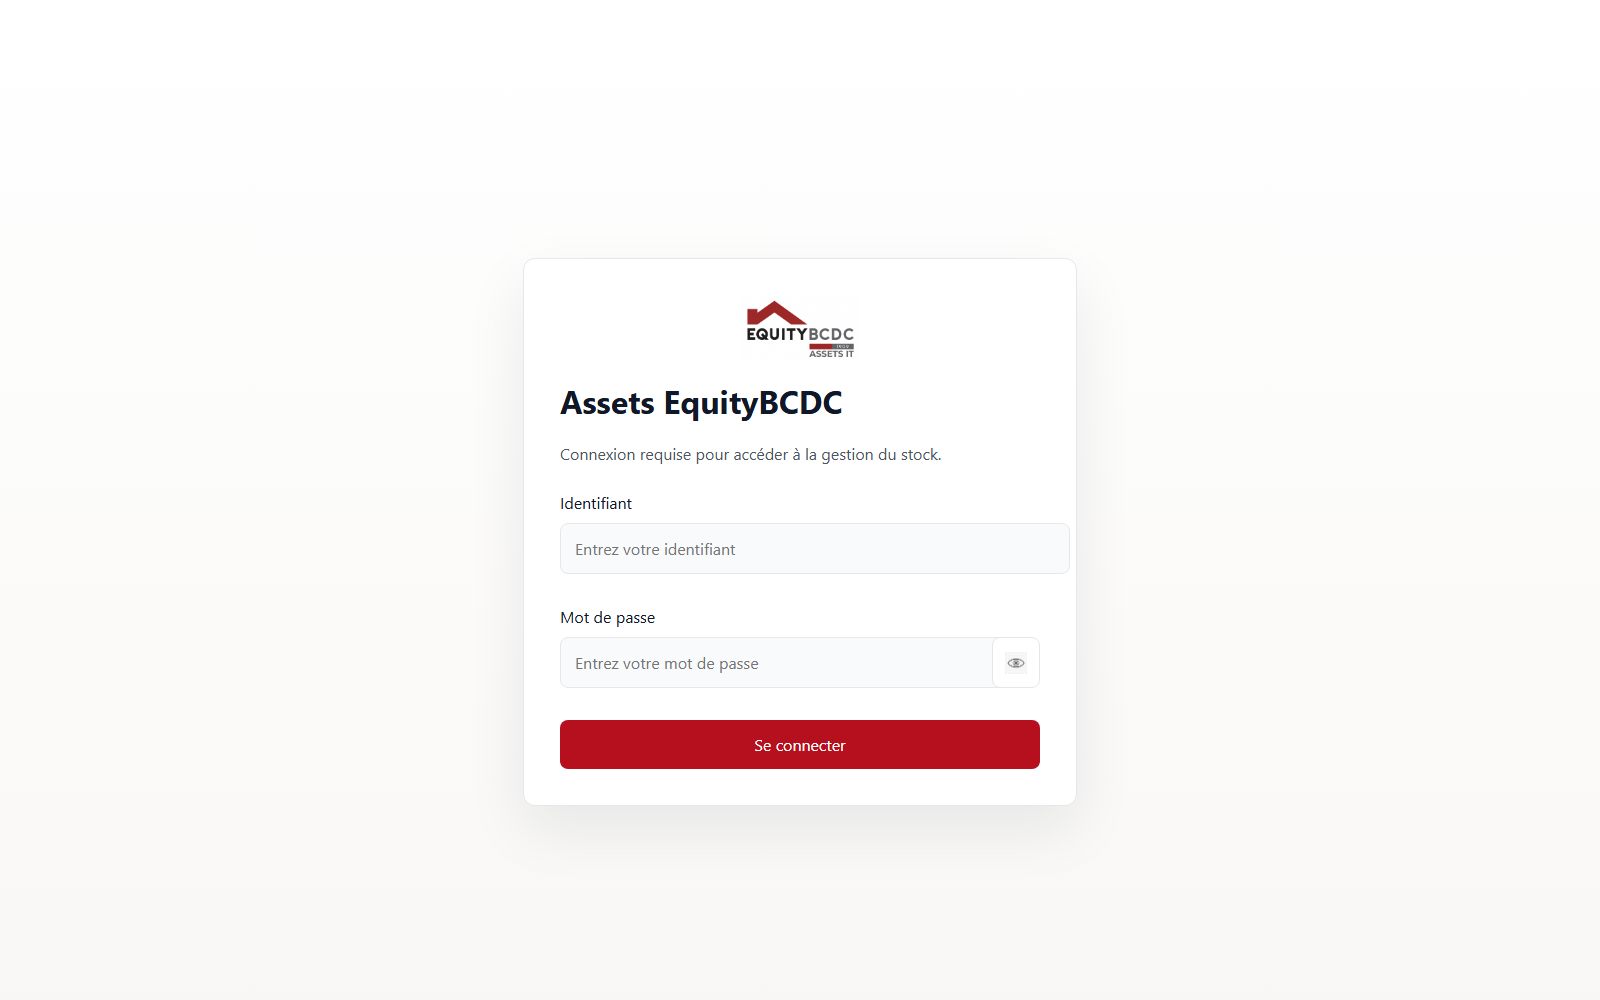
\includegraphics[width=0.95\textwidth]{01_connexion.png}
\caption{Écran de connexion de l'application Assets Equity BCDC}
\end{figure}

\begin{figure}[p]
\centering
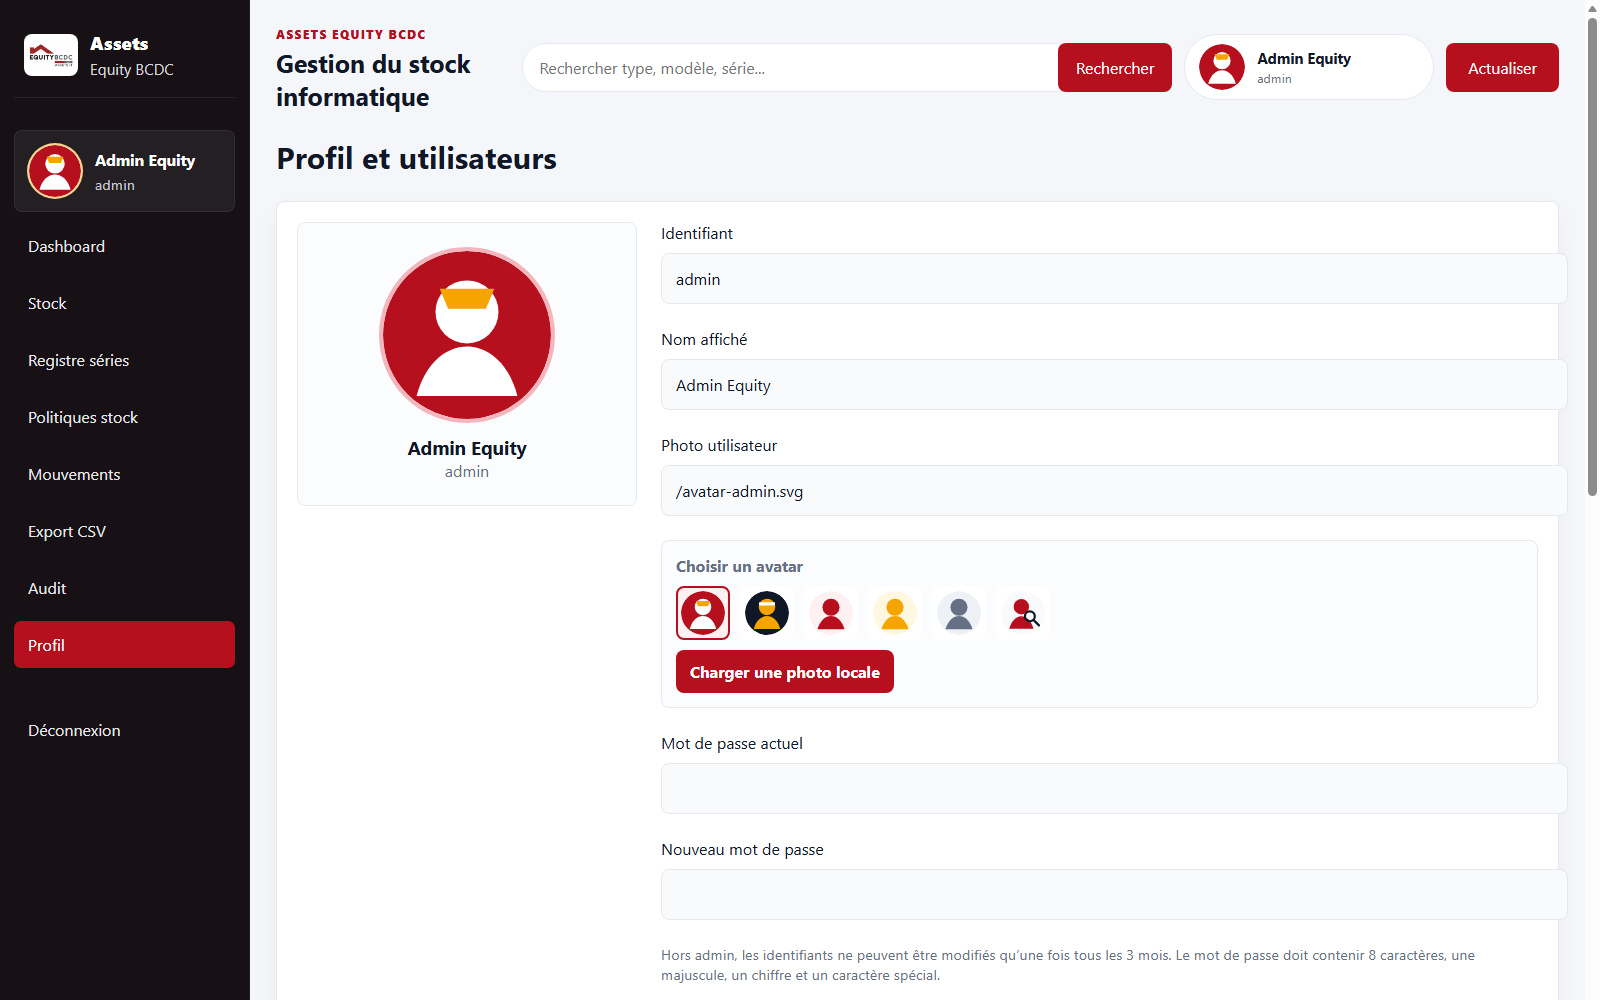
\includegraphics[width=0.95\textwidth]{09_profil.png}
\caption{Écran de profil utilisateur}
\end{figure}

\subsection{Fonctionnalités principales}

Les principales fonctionnalités développées sont les suivantes :

\begin{itemize}[label=--]
    \item authentification des utilisateurs par identifiant et mot de passe ;
    \item tableau de bord présentant le stock total, les entrées, les sorties, les séries disponibles et les alertes ;
    \item enregistrement des entrées de matériel avec type, quantité, description et numéros de série pour les équipements traçables ;
    \item import de numéros de série depuis un fichier CSV ou XLS pour accélérer la saisie des lots ;
    \item enregistrement des sorties uniquement à partir d'un matériel disponible en stock ;
    \item obligation de renseigner la destination et la personne qui prend le matériel lors d'une sortie ;
    \item registre des numéros de série indiquant les matériels encore en stock et ceux déjà sortis ;
    \item calcul automatique du stock à partir des mouvements d'entrée et de sortie ;
    \item prévision des risques de pénurie à partir de la consommation récente ;
    \item export CSV des mouvements pour les responsables autorisés ;
    \item journal d'audit des actions sensibles.
\end{itemize}

\begin{figure}[p]
\centering
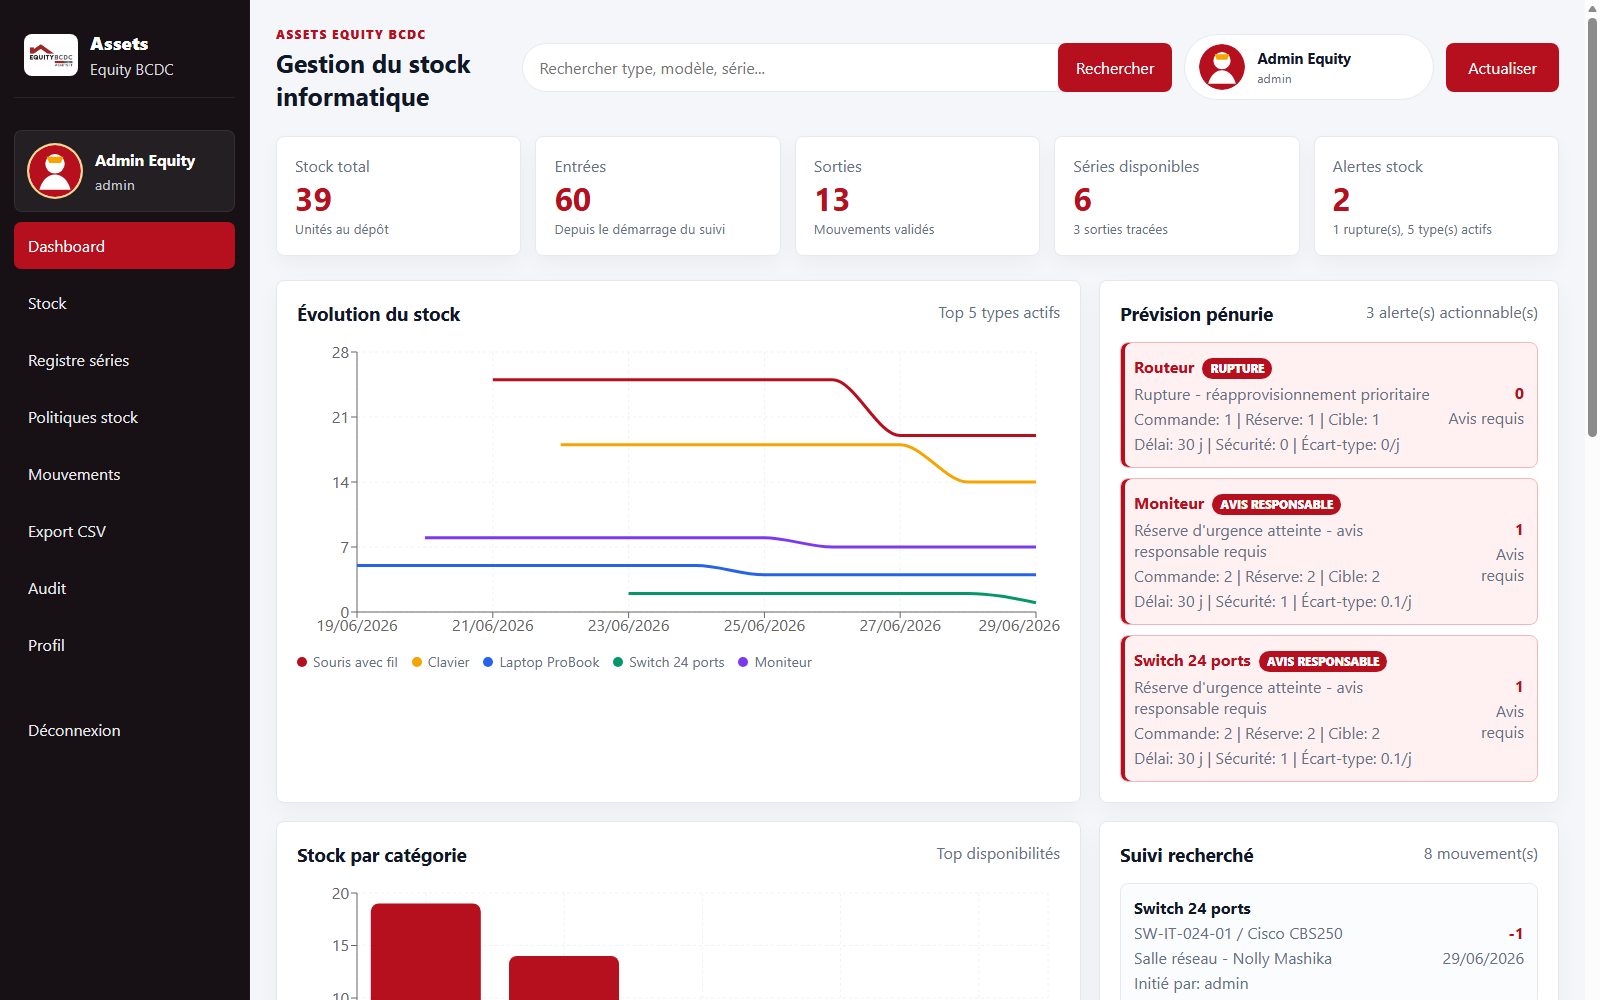
\includegraphics[width=0.95\textwidth]{02_tableau_de_bord.png}
\caption{Tableau de bord de suivi du stock informatique}
\end{figure}

\subsection{Données gérées}

Le modèle de données de l'application repose sur plusieurs entités. La table des utilisateurs conserve les comptes autorisés, les rôles, le statut du compte et la photo de profil. Le référentiel des types d'équipements contient les catégories suivies, par exemple les desktops, laptops, moniteurs, switchs, routeurs, scanners, souris, claviers, câbles, chargeurs et autres accessoires. La table des matériels représente les équipements enregistrés, tandis que la table des mouvements conserve toutes les entrées et sorties.

Pour les matériels traçables individuellement, une table spécifique des numéros de série permet de distinguer les équipements encore disponibles de ceux déjà sortis. L'application utilise aussi des politiques de stock par type de matériel, avec le délai fournisseur, le nombre de jours de réserve d'urgence, le stock minimum, la couverture cible et le facteur de service. Enfin, une table d'audit enregistre les actions importantes : connexions, créations de mouvements, exports, modifications d'utilisateurs et opérations nécessitant un avis responsable.

\begin{figure}[p]
\centering
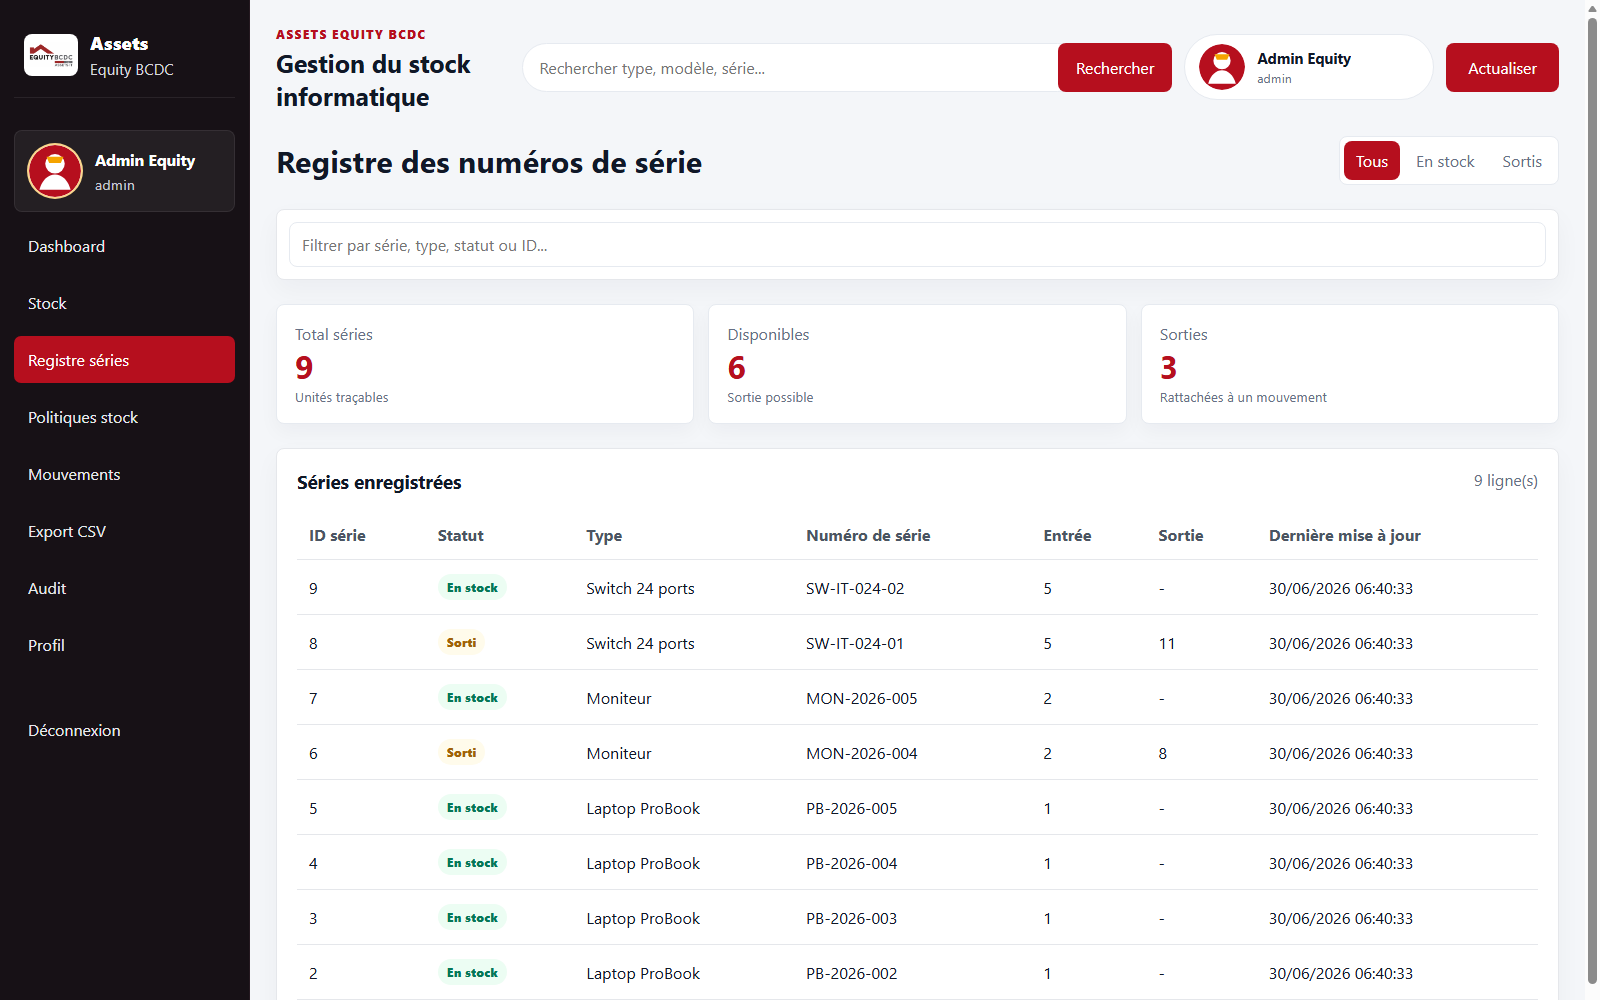
\includegraphics[width=0.95\textwidth]{04_registre_series.png}
\caption{Registre des numéros de série des équipements}
\end{figure}

\subsection{Architecture technique}

L'architecture retenue est une architecture web client-serveur simple. Le backend est développé en Python avec FastAPI. Il expose les services d'authentification, d'inventaire, de mouvements, de prévision, d'export et d'audit. Le frontend est développé avec React et Vite. Il fournit les écrans utilisés par les agents : tableau de bord, gestion des entrées et sorties, registre des séries, politiques de stock, audit, export et profil utilisateur.

La base de données principale prévue est MySQL. Pour faciliter les tests locaux, l'application peut aussi fonctionner avec SQLite lorsqu'aucune chaîne de connexion MySQL n'est configurée. La mise à jour de l'interface est renforcée par un mécanisme WebSocket permettant de rafraîchir les indicateurs après une opération de stock.

\begin{figure}[h!]
\centering
\begin{tikzpicture}[
    node distance=0.8cm,
    box/.style={draw, rounded corners, align=center, minimum width=2.8cm, minimum height=1cm, fill=gray!8},
    arrow/.style={-{Latex[length=3mm]}, thick}
]
\node[box] (user) {Utilisateur\\navigateur};
\node[box, right=of user] (frontend) {Frontend\\React/Vite};
\node[box, right=of frontend] (backend) {Backend\\FastAPI};
\node[box, right=of backend] (db) {Base de données\\MySQL ou SQLite};
\node[box, below=of backend] (audit) {Audit, logs\\et exports CSV};
\draw[arrow] (user) -- (frontend);
\draw[arrow] (frontend) -- node[above]{API REST / WebSocket} (backend);
\draw[arrow] (backend) -- (db);
\draw[arrow] (backend) -- (audit);
\end{tikzpicture}
\caption{Architecture simplifiée de l'application Assets Equity BCDC}
\end{figure}

\subsection{Cycle de gestion d'un équipement}

L'application s'inscrit dans le processus général de gestion d'un actif informatique. Ce processus peut être représenté de la manière suivante :

\begin{figure}[h!]
\centering
\begin{tikzpicture}[
    step/.style={draw, rounded corners, align=center, minimum width=2.4cm, minimum height=0.9cm, fill=blue!6},
    arrow/.style={-{Latex[length=3mm]}, thick}
]
\node[step] (reception) {Réception};
\node[step, right=0.55cm of reception] (record) {Enregistrement};
\node[step, right=0.55cm of record] (stock) {Stockage};
\node[step, right=0.55cm of stock] (assign) {Affectation};
\node[step, below=0.9cm of assign] (move) {Mouvement};
\node[step, left=0.55cm of move] (maint) {Maintenance};
\node[step, left=0.55cm of maint] (retire) {Retrait};
\draw[arrow] (reception) -- (record);
\draw[arrow] (record) -- (stock);
\draw[arrow] (stock) -- (assign);
\draw[arrow] (assign) -- (move);
\draw[arrow] (move) -- (maint);
\draw[arrow] (maint) -- (retire);
\end{tikzpicture}
\caption{Cycle de vie simplifié d'un équipement informatique}
\end{figure}

\subsection{Règles métier implémentées}

Le stock courant n'est pas saisi manuellement. Il est calculé à partir du journal des mouvements selon la règle :

\[
\text{stock actuel} = \sum \text{entrées} - \sum \text{sorties}
\]

Cette approche limite les incohérences, car chaque quantité affichée peut être expliquée par l'historique des mouvements. Pour une entrée, l'utilisateur renseigne le type de matériel, la quantité et une description. Pour les équipements traçables, comme les laptops, desktops, moniteurs, routeurs ou switchs, les numéros de série sont obligatoires afin d'éviter les doublons.

Pour une sortie, l'application impose le choix d'un matériel déjà disponible. Elle bloque donc la sortie d'un équipement inexistant ou insuffisant en stock. Elle exige également la destination, la personne qui prend le matériel, le modèle et le numéro de série lorsque le matériel est traçable.

\begin{figure}[p]
\centering
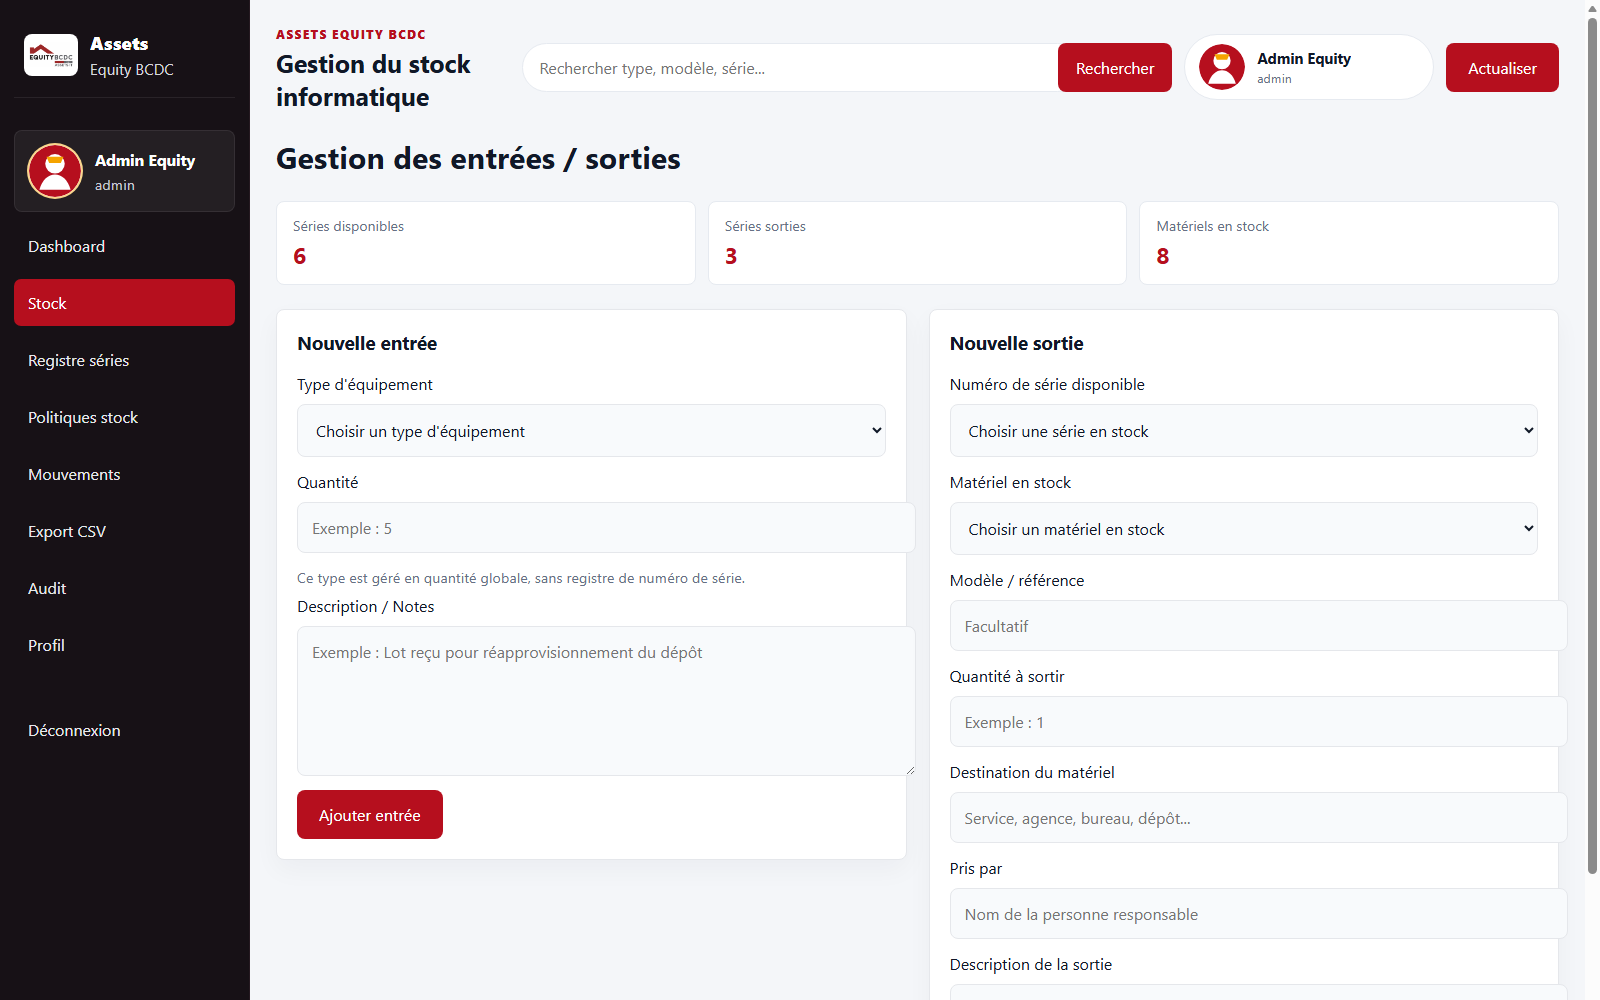
\includegraphics[width=0.95\textwidth]{03_gestion_entrees_sorties.png}
\caption{Écran de gestion des entrées et sorties de matériel}
\end{figure}

\begin{figure}[p]
\centering
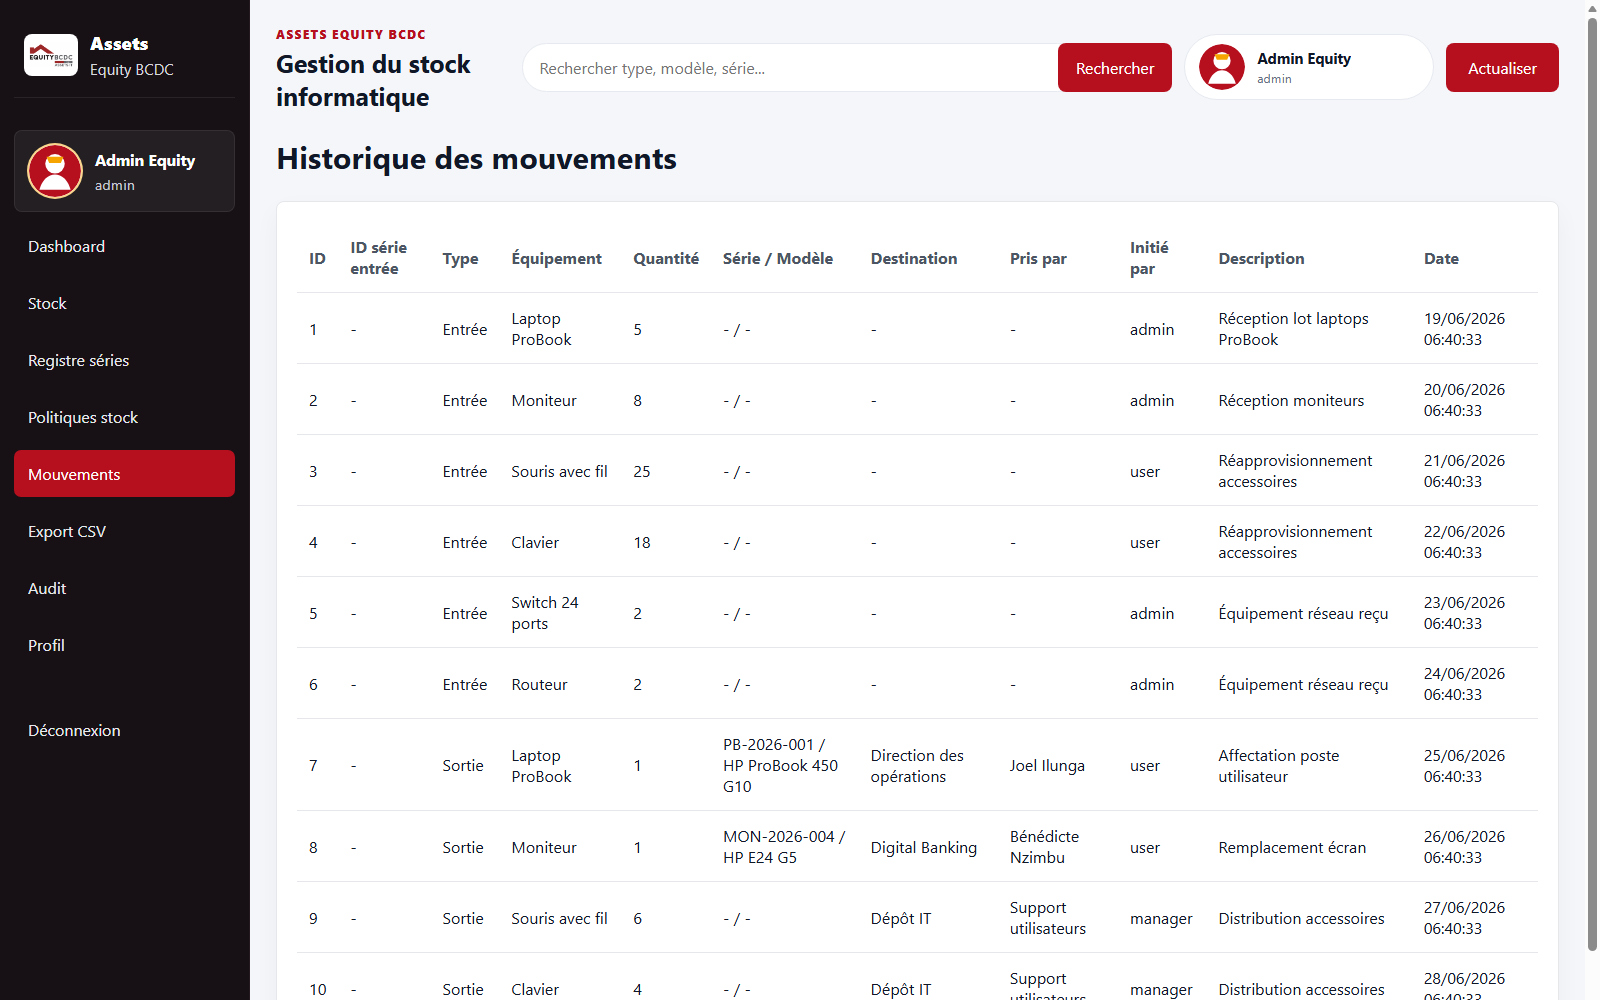
\includegraphics[width=0.95\textwidth]{06_mouvements.png}
\caption{Historique des mouvements de stock}
\end{figure}

\subsection{Prévision et alertes de stock}

L'application calcule une consommation moyenne journalière sur les 90 derniers jours :

\[
\text{consommation moyenne journalière} = \frac{\text{sorties des 90 derniers jours}}{90}
\]

Cette valeur permet d'estimer le nombre de jours avant rupture et de déterminer des seuils de commande. Les paramètres utilisés sont notamment le délai fournisseur, le stock minimum, la réserve d'urgence et le facteur de service. Lorsque le stock atteint un niveau critique, l'application signale qu'un avis responsable est requis. Cette logique transforme la recommandation générale de suivi de stock en un mécanisme technique mesurable.

\begin{figure}[p]
\centering
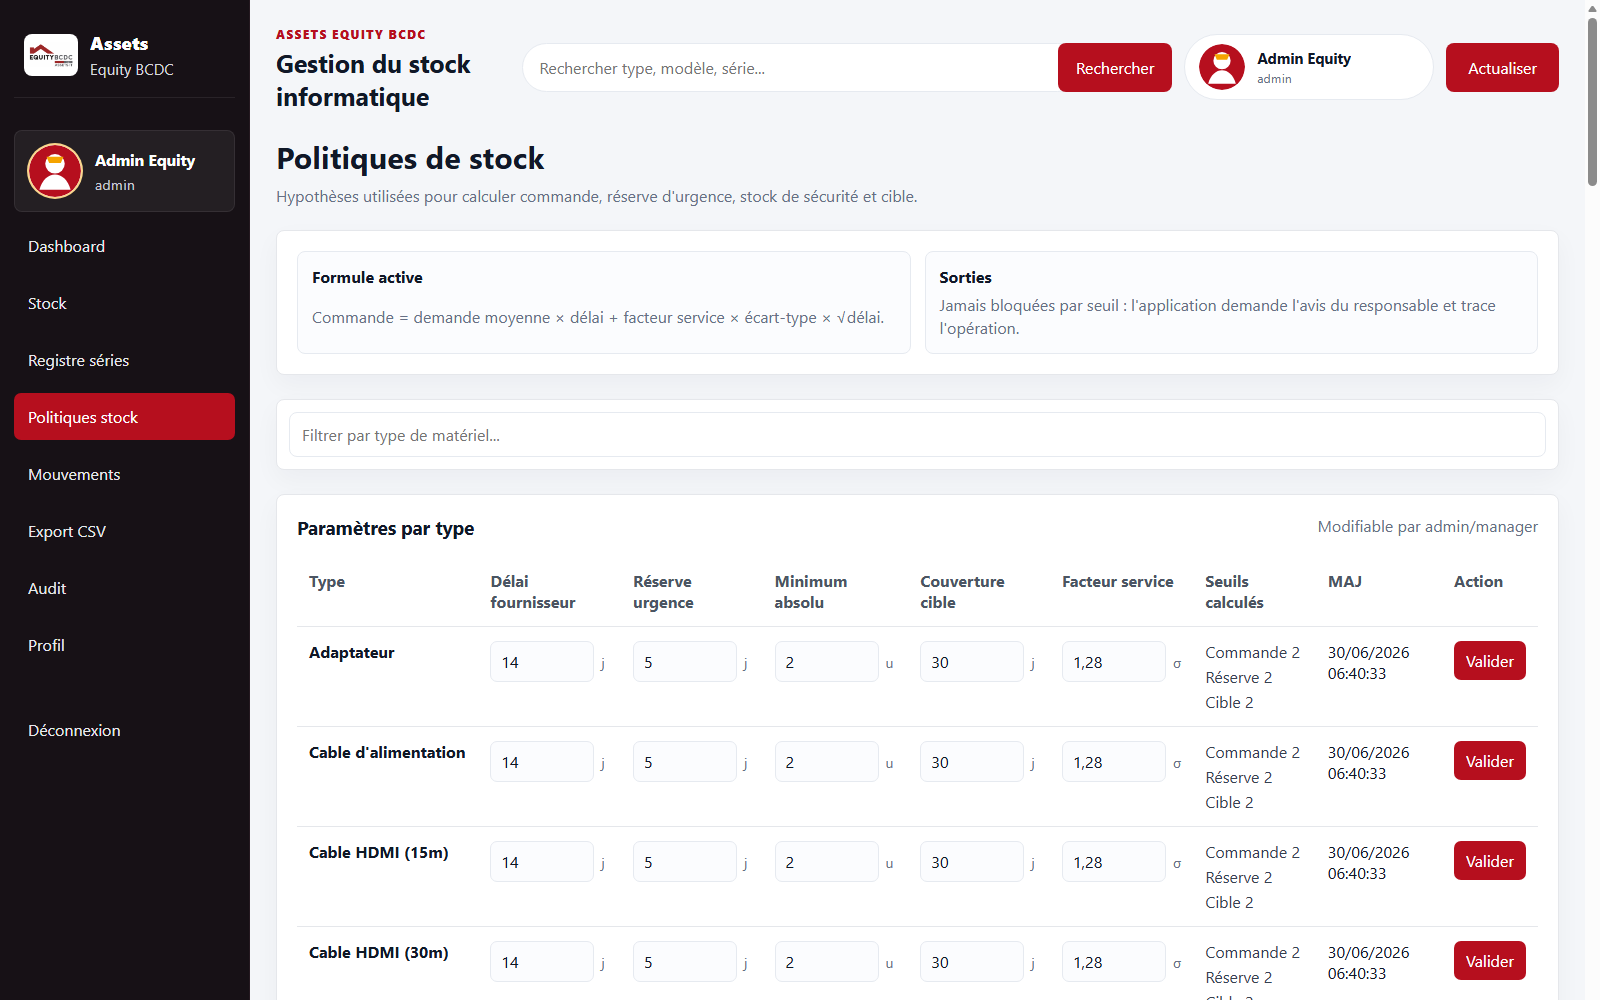
\includegraphics[width=0.95\textwidth]{05_politiques_stock.png}
\caption{Paramétrage des politiques de stock par type de matériel}
\end{figure}

\subsection{Sécurité et traçabilité}

L'application intègre plusieurs éléments adaptés à un contexte bancaire : authentification obligatoire, politique de mot de passe, rôles applicatifs, restriction des exports, journalisation des actions sensibles et table d'audit. Chaque mouvement conserve l'utilisateur connecté qui l'a initié, ce qui permet de répondre à des questions essentielles : quel matériel a été déplacé, quand, vers quelle destination, pour quelle personne et par quel agent.

Les données manipulées restent internes : comptes utilisateurs, numéros de série, destinations, bénéficiaires, historiques de mouvements et statistiques de stock. Leur accès doit donc être limité aux personnes autorisées, avec une mise en production sécurisée par HTTPS, sauvegardes contrôlées et gestion rigoureuse des identifiants.

\begin{figure}[p]
\centering
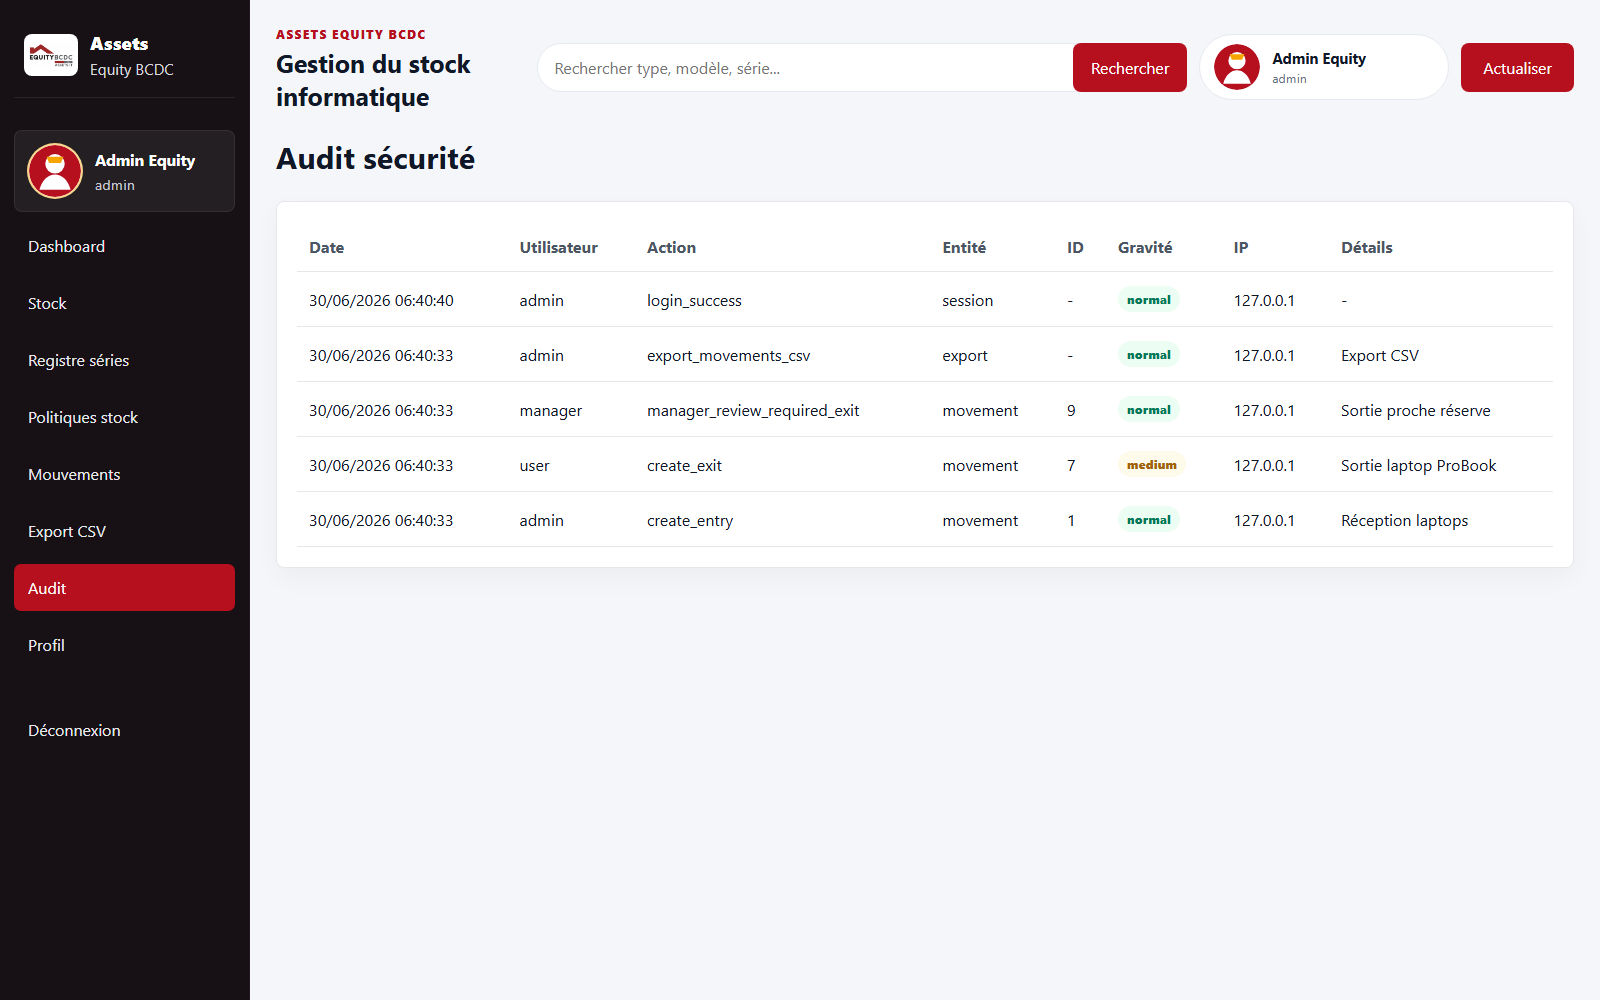
\includegraphics[width=0.95\textwidth]{08_audit.png}
\caption{Journal d'audit des actions sensibles}
\end{figure}

\begin{figure}[p]
\centering
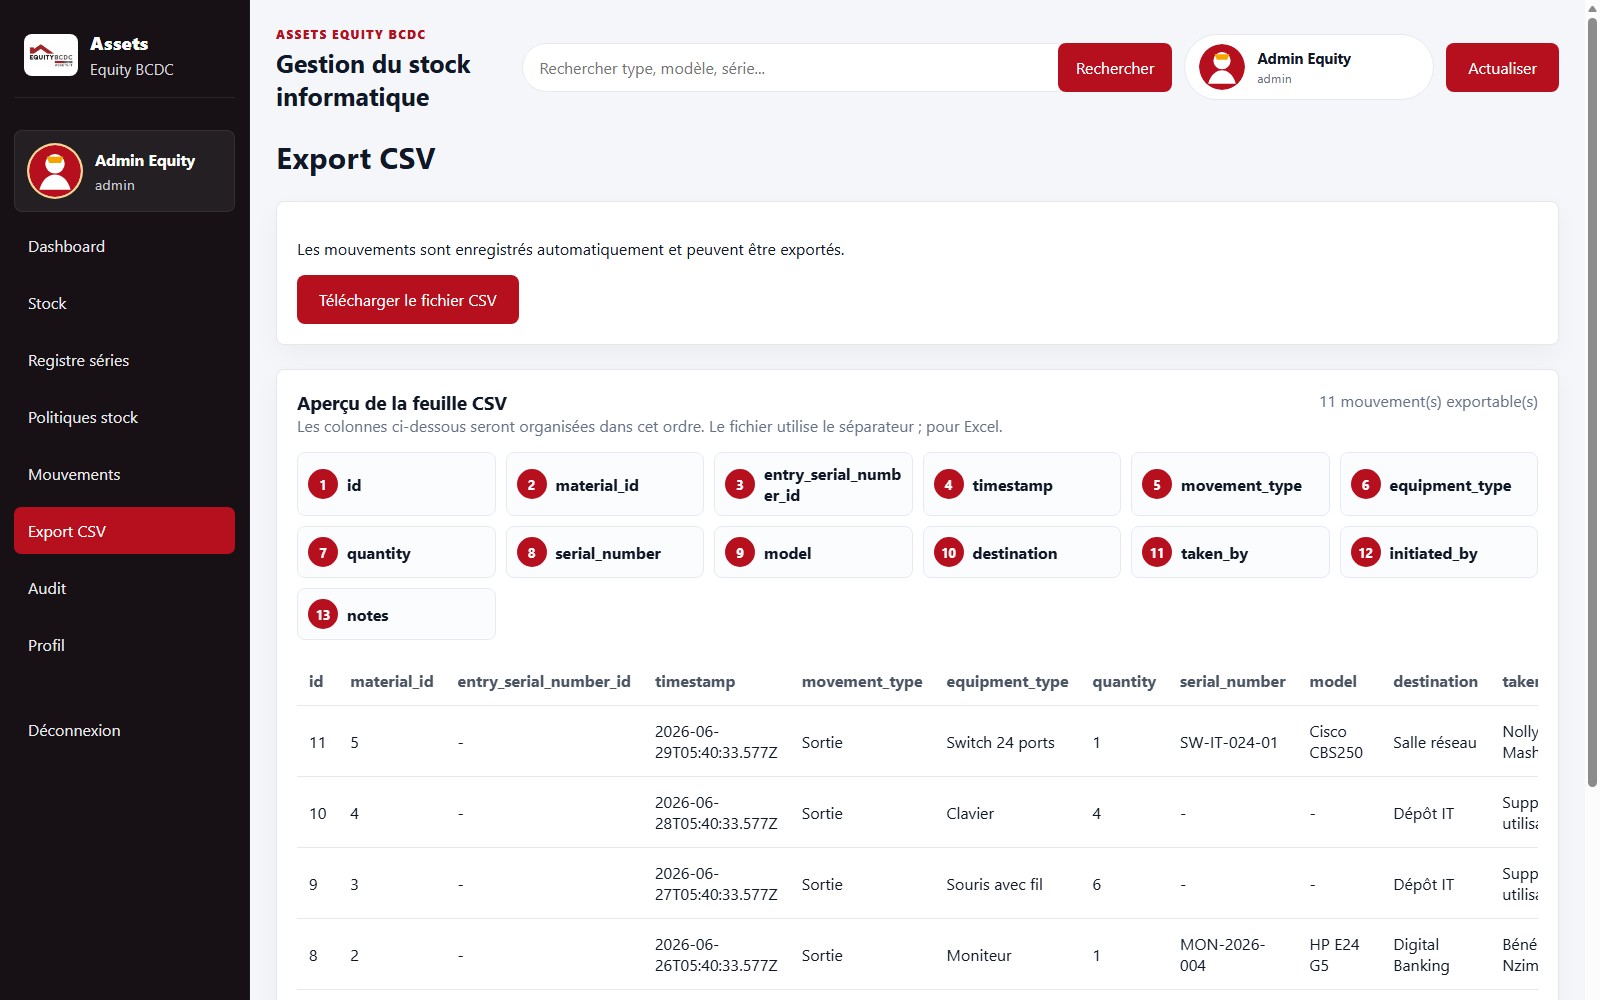
\includegraphics[width=0.95\textwidth]{07_export_csv.png}
\caption{Écran d'export des mouvements de stock}
\end{figure}

\section{Immersion dans les différentes directions de l'entreprise}

Les opérations d'inventaire ont nécessité des déplacements dans plusieurs bureaux et directions de l'entreprise. Cette mobilité m'a permis de mieux comprendre l'organisation interne de la banque et le rôle de certaines fonctions; entre autres les services liés à la digitalisation, aux opérations et à l'Information Security.

La fonction de digitalisation occupe une place importante dans la modernisation des services bancaires d'EquityBCDC. Elle vise à développer des solutions numériques permettant aux clients d'accéder aux services financiers à distance, notamment à travers les solutions mobiles, le Web Banking, l'USSD, les transferts entre portefeuilles électroniques et comptes bancaires, ainsi que les solutions de paiement comme EquityPay.\footnote{EquityBCDC, \textit{Rapport annuel 2023}, section « Les initiatives stratégiques de la banque ». Le rapport indique qu'EquityBCDC poursuit sa stratégie de numérisation des services et de développement des produits digitaux afin de rendre les clients autonomes dans leurs transactions via les solutions mobiles et le Web Banking. Disponible sur : \url{https://equitygroupholdings.com/cd/media/fg1d2qzc/equitybcdc_rapport_annuel_2023_fr_web.pdf}. Consulté le 25 juin 2026.}


La Direction des opérations assure la coordination et le suivi des processus opérationnels nécessaires à l'exécution des services bancaires. Elle intervient notamment dans le traitement des opérations de la clientèle, la gestion des flux transactionnels, l'efficacité du back-office
et l'amélioration de la qualité de service.\footnote{EquityBCDC, \textit{Rapport annuel 2024},
section « Le Comité de Direction », où figure le Directeur des opérations. Le même rapport souligne que le développement des services d'appui partagés contribue à consolider les activités de back-office, à améliorer la productivité et l'expérience client. Disponible sur :
\url{https://equitygroupholdings.com/cd/media/rc0g53dh/31907_equitybcdc_rapport_annuel_2024_fr_web.pdf}. Consulté le 25 juin 2026.}

Le département INFOSEC, ou Information Security, est chargé de la protection
des informations, des systèmes et des actifs numériques de la banque. Il intervient notamment dans la gestion des risques liés à la technologie, à l'information et à la cybersécurité, la gestion des accès, la sécurité des applications, la réponse aux incidents et la sensibilisation du personnel.\footnote{EquityBCDC,\textit{Rapport Pilier III au 31 décembre 2024}, section « Gestion du risque informatique ».
Disponible sur : \url{https://equitygroupholdings.com/cd/media/g0obofud/rapport_pilier_31_dec_2024_ok-2.pdf}. Consulté le 25 juin 2026.}

Cette immersion m'a permis de comprendre que le service IT-Asset Management est transversal. Il fournit ou suit les équipements utilisés par plusieurs directions. Son efficacité influence donc indirectement la qualité de travail d'autres services.

\section{Méthodes de travail observées}

Durant le stage, plusieurs méthodes de travail ont été observées.
La première est la vérification systématique. Les informations collectées doivent être exactes, notamment les numéros de série et les affectations.
La deuxième est la documentation des opérations. Les mouvements de matériel, les commandes, les entrées et les sorties de stock doivent être enregistrés afin de conserver une trace exploitable.
La troisième est la coordination avec les utilisateurs. Les opérations d'inventaire nécessitent de communiquer avec les agents, d'accéder à leurs postes et de réaliser les relevés sans perturber excessivement leur travail.
La quatrième est le respect des procédures internes. Dans une banque, les activités informatiques ne peuvent pas être réalisées de manière informelle. Elles doivent suivre des règles précises afin de garantir la sécurité, la responsabilité et la conformité.

Ces méthodes de travail m'ont permis de comprendre que l'efficacité d'un service informatique dépend autant des compétences techniques que de l'organisation interne.

% =========================================================
% CHAPITRE 3
% =========================================================
\chapter{Difficultés, acquis et suggestions}

\section{Difficultés rencontrées}

Le stage s'est déroulé dans de bonnes conditions, mais certaines difficultés ont été observées.

La première difficulté concernait l'indisponibilité ponctuelle de certains équipements ou accessoires demandés par les utilisateurs. Il pouvait s'agir d'ordinateurs, de souris, de claviers, de câbles ou d'autres matériels nécessaires au travail quotidien. Cette situation pouvait entraîner des retards dans la prise en charge de certaines demandes.
La deuxième difficulté était liée à la précision exigée lors de l'inventaire. Le relevé des numéros de série demande une attention particulière. Certains numéros peuvent être difficiles à lire selon l'emplacement de l'étiquette, l'état du matériel ou les conditions d'accès au poste.
La troisième difficulté concernait la nécessité de réaliser les opérations d'inventaire sans perturber les agents dans leur travail. Il fallait donc intervenir avec méthode, rapidité, courtoisie et patience si nécessaire.
La quatrième difficulté était liée à l'adaptation progressive aux procédures internes notamment les règles de fonctionnement du service, les circuits de validation et les exigences propres à l'environnement bancaire.

Ces difficultés ont constitué des situations d'apprentissage. Elles m'ont permis de développer une approche plus rigoureuse, plus organisée et plus attentive aux contraintes du terrain.

\section{Compétences techniques acquises}

Le stage m'a permis de développer plusieurs compétences techniques liées à la gestion des actifs informatiques.
J'ai appris à participer à un inventaire physique d'équipements informatiques. Cette compétence consiste à identifier correctement un matériel, à relever ses informations essentielles et à vérifier son affectation.
J'ai compris l'importance du numéro de série comme identifiant unique d'un équipement. Cette information, négligée dans un usage domestique, joue un rôle central dans la traçabilité, la maintenance, les contrôles et la gestion du parc.
J'ai également découvert les principes de gestion des stocks informatiques. Le suivi des entrées et sorties permet de connaître les quantités disponibles, d'anticiper les besoins et de réduire les délais de prise en charge.
J'ai été initié à l'enregistrement des bons de commande, qui assure le lien entre les achats réalisés et les matériels réceptionnés.
Enfin, j'ai observé les étapes de préparation des postes de travail avant leur affectation aux utilisateurs. Cette observation m'a permis de comprendre les exigences minimales de configuration, de mise à jour et de contrôle avant la mise en service d'un équipement.

Dans le but d'évaluer ma compréhension du travail fait dans le service, j'ai implémenté une application d'aide à la gestion des entrées et sorties d'équipements. Cette réalisation m'a permis de traduire un besoin métier en modèle de données, en règles de validation et en écrans exploitables par un utilisateur.

Sur le plan technique, j'ai appris à structurer les données autour des entités essentielles : utilisateurs, types d'équipements, matériels, numéros de série, mouvements, politiques de stock et journaux d'audit. J'ai également compris l'intérêt de calculer le stock à partir des mouvements plutôt que de modifier directement une quantité globale. Cette méthode rend les chiffres plus vérifiables, car chaque variation de stock correspond à une opération enregistrée.

Le développement de l'application m'a aussi permis de mettre en pratique des notions de sécurité applicative : authentification obligatoire, politique de mot de passe, rôles d'accès, restriction des exports et traçabilité des actions sensibles. Ces éléments sont importants dans une institution bancaire où même les données de stock informatique doivent rester contrôlées.

\section{Compétences professionnelles acquises}

Au-delà des aspects techniques, le stage m'a permis de développer des compétences professionnelles importantes.
La rigueur a été nécessaire dans la collecte et l'enregistrement des informations. Une erreur sur un numéro de série ou une affectation peut produire des incohérences dans le suivi du matériel.
Le sens de l'organisation a été renforcé par les activités de stock et d'inventaire. Ces tâches nécessitent une méthode claire et une gestion ordonnée des informations.
Le travail en équipe a été développé grâce à l'accompagnement reçu et aux activités réalisées avec les agents du service. J'ai compris qu'un service informatique fonctionne efficacement lorsque les tâches sont coordonnées et les informations partagées.
La communication a également été importante. Les opérations d'inventaire impliquent des échanges avec les utilisateurs, les responsables de service et les membres de l'équipe informatique.

Enfin, le stage m'a permis de développer une meilleure compréhension du comportement exigé dans un environnement professionnel : ponctualité, respect des consignes, discrétion, responsabilité et adaptation.

\section{Analyse critique}

L'expérience effectuée au sein du service IT-Asset Management montre que la gestion des actifs informatiques est une fonction stratégique dans une institution bancaire.

Un parc informatique mal maîtrisé peut créer plusieurs problèmes : perte d'équipements, doublons dans les achats, retard dans les affectations, difficulté de maintenance, manque de visibilité sur les stocks et faiblesse lors des contrôles internes.

À l'inverse, une bonne gestion des actifs permet de disposer d'une vision claire du patrimoine informatique. Elle facilite les décisions d'achat, améliore la disponibilité des équipements, réduit les pertes et soutient la continuité des opérations.

Dans une logique d'ingénierie, le service IT-Asset Management peut être considéré comme un système de contrôle du patrimoine matériel. Il collecte des données, les organise, les met à jour et les exploite pour assurer le bon fonctionnement de l'environnement informatique.

Cependant, l'efficacité de ce système dépend de plusieurs facteurs : la qualité des données, la régularité des inventaires, la discipline dans l'enregistrement des mouvements, la disponibilité des outils de suivi et la collaboration des utilisateurs.

Les problèmes observés peuvent être regroupés en trois catégories. La première concerne la qualité des données : un numéro de série mal saisi, absent ou enregistré deux fois rend l'identification d'un équipement difficile. La deuxième concerne la disponibilité du stock : sans seuils clairs, certaines ruptures peuvent être constatées trop tard. La troisième concerne la traçabilité : lorsque les mouvements ne sont pas enregistrés de manière uniforme, il devient plus difficile de reconstituer l'historique d'un matériel.

L'application développée apporte une réponse partielle à ces problèmes. Elle impose certaines validations, conserve l'historique des mouvements, associe chaque action à un utilisateur connecté et calcule des alertes à partir de paramètres de stock. Toutefois, pour une adoption complète, elle devrait être intégrée aux procédures internes, testée avec des données réelles autorisées et accompagnée d'une formation des utilisateurs.

Le stage a donc montré que la gestion des actifs informatiques ne doit pas être considérée comme une simple activité administrative. Elle est liée à la gouvernance informatique, à la sécurité, à la continuité de service et à l'optimisation des ressources.

\section{Suggestions et recommandations}

À partir des observations faites durant le stage, les recommandations suivantes peuvent être formulées par ordre de priorité.

\subsection{Priorité 1 : déployer un outil interne de gestion des actifs}

La principale recommandation consiste à mettre en place un outil interne dédié au suivi du parc matériel. L'application développée, \textit{Assets Equity BCDC}, constitue une base technique pouvant être améliorée et adaptée aux procédures internes.

La proposition technique repose sur les modules suivants :

\begin{itemize}[label=--]
    \item \textbf{module d'authentification} : connexion nominative, rôles, expiration des sessions et politique de mot de passe ;
    \item \textbf{module inventaire} : enregistrement des matériels, types d'équipements, numéros de série et états ;
    \item \textbf{module mouvements} : gestion des entrées, sorties, affectations, destinations et bénéficiaires ;
    \item \textbf{module demandes} : réception et suivi des demandes de matériel formulées par les employés ;
    \item \textbf{module registre des séries} : suivi des équipements traçables individuellement ;
    \item \textbf{module politiques de stock} : seuil de commande, réserve d'urgence, délai fournisseur et stock minimum ;
    \item \textbf{module tableau de bord} : indicateurs, courbes d'évolution, alertes de pénurie et mouvements récents ;
    \item \textbf{module audit et export} : journal des actions sensibles et export CSV réservé aux profils autorisés.
\end{itemize}

Les données à stocker doivent inclure au minimum : type d'équipement, numéro de série, modèle, quantité, destination, personne bénéficiaire, utilisateur initiateur, date du mouvement, rôle utilisateur, seuils de stock et observations. Une telle structuration permettrait de réduire les écarts entre le matériel enregistré et le matériel réellement disponible.

\subsection{Priorité 2 : formaliser une procédure d'inventaire}

Il est recommandé de documenter une procédure d'inventaire commune à toutes les équipes concernées. Cette procédure devrait préciser les champs obligatoires, la méthode de vérification du numéro de série, la manière de signaler un matériel non identifié et les règles de correction en cas de doublon.

Une fiche standard d'actif informatique devrait accompagner cette procédure. Elle faciliterait la collecte sur le terrain et l'intégration des données dans l'outil de suivi.

\subsection{Priorité 3 : définir des seuils de stock par type de matériel}

Les accessoires et équipements les plus sollicités doivent disposer de seuils de commande. Le seuil ne devrait pas être choisi uniquement de manière fixe ; il devrait tenir compte de la consommation récente, du délai fournisseur, du stock minimum et de la criticité du matériel.

L'application développée applique déjà cette logique en calculant une consommation moyenne journalière sur les 90 derniers jours et en comparant le stock courant avec un seuil de commande et une réserve d'urgence. Cette approche peut aider le service à passer d'une gestion réactive à une gestion plus préventive.

\subsection{Priorité 4 : mettre en place une plateforme de demandes de matériel}

Il serait également pertinent de mettre en place une plateforme interne permettant aux employés de formuler leurs demandes de matériel sans devoir se déplacer systématiquement jusqu'au service IT-Asset Management. Cette plateforme pourrait être intégrée à l'outil de gestion des actifs ou fonctionner comme un module complémentaire relié au stock.

Le principe serait simple : l'utilisateur soumet une demande en précisant le type de matériel souhaité, le motif, la direction concernée, le niveau d'urgence et les informations utiles à la prise en charge. La demande serait ensuite reçue par le service IT-Asset Management, qui pourrait vérifier la disponibilité du matériel, valider ou rejeter la demande, préparer l'équipement et enregistrer la sortie si la demande est approuvée.

Une telle plateforme présenterait plusieurs avantages. Elle réduirait les déplacements inutiles des employés, améliorerait la traçabilité des demandes, faciliterait la priorisation des besoins et permettrait au service IT-Asset Management de disposer d'un historique exploitable. Elle contribuerait aussi à mieux distinguer les demandes urgentes, les demandes ordinaires, les remplacements et les besoins liés à de nouvelles affectations.

Sur le plan technique, ce module pourrait contenir les données suivantes : demandeur, direction, type de matériel demandé, motif, priorité, statut de la demande, date de création, agent traitant, décision prise et commentaire de clôture. Les statuts possibles pourraient être : en attente, en cours d'analyse, approuvée, rejetée, matériel préparé et clôturée.

\subsection{Priorité 5 : renforcer la sensibilisation des utilisateurs}

Outre cet outil de gestion, il serait nécessaire de sensibiliser les utilisateurs à la bonne conservation des équipements mis à leur disposition. La gestion des actifs ne dépend pas uniquement du service informatique. Elle implique aussi les utilisateurs, qui doivent signaler les pannes, les déplacements ou les pertes.

\subsection{Priorité 6 : aligner les pratiques avec les référentiels ITAM}

Enfin, il serait utile d'aligner progressivement les pratiques internes avec les référentiels reconnus en gestion des actifs informatiques. Les normes relatives à l'IT Asset Management insistent sur la nécessité d'un système structuré, documenté et continuellement amélioré.\footnote{ISO/IEC 19770-1:2017 précise les exigences d'un système de gestion des actifs informatiques dans le contexte de l'organisation : \url{https://www.iso.org/standard/68531.html}.}

Ces recommandations visent à renforcer la fiabilité du suivi, la disponibilité du matériel, la qualité des données et la qualité du service rendu aux utilisateurs internes.

% =========================================================
% CONCLUSION
% =========================================================
\chapter*{Conclusion générale}
\addcontentsline{toc}{chapter}{Conclusion générale}

Le stage académique effectué au sein d'Equity BCDC, à la Direction Informatique et plus précisément dans le service IT-Asset Management, a constitué une expérience importante dans mon parcours de formation.

Il m'a permis de découvrir le fonctionnement d'un service informatique dans une grande institution bancaire et de comprendre le rôle de la gestion des actifs informatiques dans la continuité des activités. À travers les activités réalisées, j'ai observé que les équipements informatiques doivent être identifiés, suivis, affectés et documentés avec rigueur.

Les tâches d'inventaire, de relevé des numéros de série, de gestion des stocks, d'enregistrement des bons de commande et de préparation des postes de travail m'ont permis d'acquérir des compétences pratiques. Elles m'ont aussi montré que la performance d'un service informatique dépend fortement de la qualité des procédures et de la fiabilité des informations disponibles.

Ce stage a également renforcé ma compréhension du lien entre l'informatique et les métiers bancaires. Les équipements suivis par le service IT-Asset Management sont utilisés par plusieurs directions et soutiennent les opérations quotidiennes de l'entreprise. Leur bonne gestion contribue donc à la productivité, à la sécurité et à la qualité du service.

Les difficultés rencontrées, notamment l'indisponibilité ponctuelle de certains matériels et les exigences de précision lors de l'inventaire, ont permis de mieux comprendre les contraintes réelles du terrain. Elles ont aussi montré l'importance de la planification, de la communication et de la mise à jour régulière des données.

En définitive, cette immersion professionnelle m'a permis de relier les connaissances théoriques acquises au niveau académique aux réalités concrètes de la gestion informatique en entreprise. Elle a renforcé ma rigueur, mon sens de l'organisation, ma capacité d'analyse et ma compréhension du rôle stratégique de l'informatique dans une institution bancaire.

% =========================================================
% BIBLIOGRAPHIE
% =========================================================
\begin{thebibliography}{99}
\addcontentsline{toc}{chapter}{Bibliographie}

\bibitem{equitybcdc-accueil}
Equity BCDC, \textit{Site officiel d'Equity BCDC}. Disponible sur : \url{https://equitygroupholdings.com/cd/}. Consulté le 25 juin 2026.

\bibitem{equitybcdc-acquisition}
Equity Group Holdings, \textit{Equity Group Holdings completes acquisition of majority stake in Banque Commerciale du Congo (BCDC)}, communiqué officiel, 11 août 2020. Disponible sur : \url{https://equitygroupholdings.com/equity-group-holdings-completes-acquisition-of-majority-stake-in-banque-commerciale-du-congo-bcdc/}. Consulté le 25 juin 2026.

\bibitem{loi003}
République Démocratique du Congo, \textit{Loi n\textsuperscript{o}003/2002 du 02 février 2002 relative à l'activité et au contrôle des établissements de crédit}. Disponible sur : \url{https://www.leganet.cd/Legislation/Droit%20economique/Banques/loi.003.02.02.2002.pdf}. Consulté le 25 juin 2026.

\bibitem{bcc-loi22069}
Banque Centrale du Congo, \textit{Instruction citant la Loi n\textsuperscript{o}22/069 du 27 décembre 2022 relative à l'activité et au contrôle des établissements de crédit}. Disponible sur : \url{https://www.bcc.cd/sites/default/files/dsif/instruction_ndeg22_modification_ndeg2.pdf}. Consulté le 25 juin 2026.

\bibitem{iso19770}
ISO, \textit{ISO/IEC 19770-1:2017 -- Information technology -- IT asset management -- Part 1: IT asset management systems -- Requirements}. Disponible sur : \url{https://www.iso.org/standard/68531.html}. Consulté le 25 juin 2026.


\end{thebibliography}


\end{document}
